\chapter{Classification of Covering Spaces}

Up to this point, we have used \index{classification: of covering spaces@Classification: of covering spaces}classification covering spaces primarily as a tool for computing fundamental groups. Now we turn things around and use the fundamental group as a tool for studying covering spaces.

To do this in any reasonable way, we must restrict ourselves to the case where \(B\) is locally path connected. Once we have done this, we may as well require \(B\) to be path connected as well, since \(B\) breaks up into the disjoint open sets \({B}_{\alpha }\) that are its path components, and the maps \({p}^{-1}\left( {B}_{\alpha }\right)  \rightarrow  {B}_{\alpha }\) obtained by restricting \(p\) are covering maps, by Theorem 53.2. We may as well assume also that \(E\) is path connected. For if \({E}_{\alpha }\) is a path component of \({p}^{-1}\left( {B}_{\alpha }\right)\) , then the map \({E}_{\alpha } \rightarrow  {B}_{\alpha }\) obtained by restricting \(p\) is also a covering map. (See Lemma 80.1.) Therefore, one can determine all coverings of the locally path-connected space \(B\) merely by determining all path-connected coverings of each path component of \(B\) !

For this reason, we make the following:

Convention. Throughout this chapter, the statement that \(p : E \rightarrow  B\) is a covering map will include the assumption that \(E\) and \(B\) are locally path connected and path connected, unless specifically stated otherwise.

With this convention, we now describe the connection between covering spaces of \(B\) and the fundamental group of \(B\) .

If \(p : E \rightarrow  B\) is a covering map, with \(p\left( {e}_{0}\right)  = {b}_{0}\) , then the induced homomorphism \({p}_{ * }\) is injective, by Theorem 54.6, so that

\[
{H}_{0} = {p}_{ * }\left( {{\pi }_{1}\left( {E,{e}_{0}}\right) }\right)
\]

is a subgroup of \({\pi }_{1}\left( {B,{b}_{0}}\right)\) isomorphic to \({\pi }_{1}\left( {E,{e}_{0}}\right)\) . It turns out that the subgroup \({H}_{0}\) determines the covering \(p\) completely, up to a suitable notion of equivalence of coverings. This we shall prove in  \S 79. Furthermore, under a (fairly mild) additional ``local niceness'' condition on \(B\) , there exists, for each subgroup \({H}_{0}\) of \({\pi }_{1}\left( {B,{b}_{0}}\right)\) , a covering \(p : E \rightarrow  B\) of \(B\) whose corresponding subgroup is \({H}_{0}\) . This we shall prove in \( \S {82}\) .

Roughly speaking, these results show that one can determine all covering spaces of \(B\) merely by examining the collection of all subgroups of \({\pi }_{1}\left( {B,{b}_{0}}\right)\) . This is the classical procedure of algebraic topology; one ``solves'' a problem of topology by reducing it to a problem of algebra, hopefully one that is more tractable.

Throughout the chapter, we assume the general \index{lifting lemma: general@Lifting lemma: general}general lifting lemma lifting correspondence theorem, Theorem 54.6.

\section*{§ 79 Equivalence of Covering Spaces}

In this section, we show that the subgroup \({H}_{0}\) of \({\pi }_{1}\left( {B,{b}_{0}}\right)\) determines the covering \(p : E \rightarrow  B\) completely, up to a suitable notion of equivalence of coverings.

\begin{definition}
	Let \(p : E \rightarrow  B\) and \({p}^{\prime } : {E}^{\prime } \rightarrow  B\) be covering maps. They are said to be equivalent if there exists a homeomorphism \(h : E \rightarrow  {E}^{\prime }\) such that \(p = {p}^{\prime } \circ  h\) . The homeomorphism \(h\) is called an \index{Equivalence of covering maps}equivalence of covering maps or an equivalence of covering spaces
\end{definition}

\begin{center}
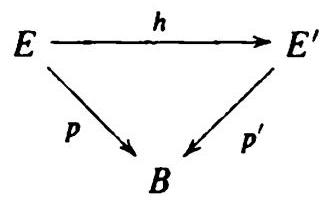
\includegraphics[width=0.3\textwidth]{images/79.0.jpg}
\end{center}
\hspace*{3em} 

Given two covering maps \(p : E \rightarrow  B\) and \({p}^{\prime } : {E}^{\prime } \rightarrow  B\) whose corresponding subgroups \({H}_{0}\) and \({H}_{0}^{\prime }\) are equal, we shall prove that there exists an equivalence \(h\) : \(E \rightarrow  {E}^{\prime }\) . For this purpose, we need to generalize the lifting lemmas of \( \S {54}\) .

\begin{lemma}[The \index{General lifting lemma}general lifting lemma]
	Let \(p : E \rightarrow  B\) be a covering map; let \(p\left( {e}_{0}\right)  = {b}_{0}\) . Let \(f : Y \rightarrow  B\) be a continuous map, with \(f\left( {y}_{0}\right)  = {b}_{0}\) . Suppose \(Y\) is path connected and locally path connected. The map \(f\) can be lifted to a map \(\widetilde{f} : Y \rightarrow  E\) such that \(\bar{f}\left( {y}_{0}\right)  = {e}_{0}\) if and only if

\[
{f}_{ * }\left( {{\pi }_{1}\left( {Y,{y}_{0}}\right) }\right)  \subset  {p}_{ * }\left( {{\pi }_{1}\left( {E,{e}_{0}}\right) }\right) .
\]

Furthermore, if such a lifting exists, it is unique.
\end{lemma}

\begin{proof}
	If the lifting \(\widetilde{f}\) exists, then
\[
{f}_{ * }\left( {{\pi }_{1}\left( {Y,{Y}_{0}}\right) }\right)  = {p}_{ * }\left( {{\bar{f}}_{ * }\left( {{\pi }_{1}\left( {Y,{y}_{0}}\right) }\right) }\right)  \subset  {p}_{ * }\left( {{\pi }_{1}\left( {E,{e}_{0}}\right) }\right) .
\]

This proves the ``only if'' part of the theorem.

Now we prove that if \(\widetilde{f}\) exists, it is unique. Given \({y}_{1} \in  Y\) , choose a path \(\alpha\) in \(Y\) from \({y}_{0}\) to \({y}_{1}\) . Take the path \(f \circ  \alpha\) in \(B\) and lift it to a path \(\gamma\) in \(E\) beginning at \({e}_{0}\) . If a lifting \(\bar{f}\) of \(f\) exists, then \(\bar{f}\left( {y}_{1}\right)\) must equal the end point \(\gamma \left( 1\right)\) of \(\gamma\) , for \(\bar{f} \circ  \alpha\) is a lifting of \(f \circ  \alpha\) that begins at \({e}_{0}\) , and path liftings are unique.

Finally, we prove the ``if'' part of the theorem. The uniqueness part of the proof gives us a clue how to proceed. Given \({y}_{1} \in  Y\) , choose a path \(\alpha\) in \(Y\) from \({y}_{0}\) to \({y}_{1}\) . Lift the path \(f \circ  \alpha\) to a path \(\gamma\) in \(E\) beginning at \({e}_{0}\) , and define \(\widetilde{f}\left( {y}_{1}\right)  = \gamma \left( 1\right)\) . See Figure 79.1. It is a certain amount of work to show that \(\widetilde{f}\) is well-defined, independent of the choice of \(\alpha\) . Once we prove that, continuity of \(\widetilde{f}\) is proved easily, as we now show.

\begin{center}
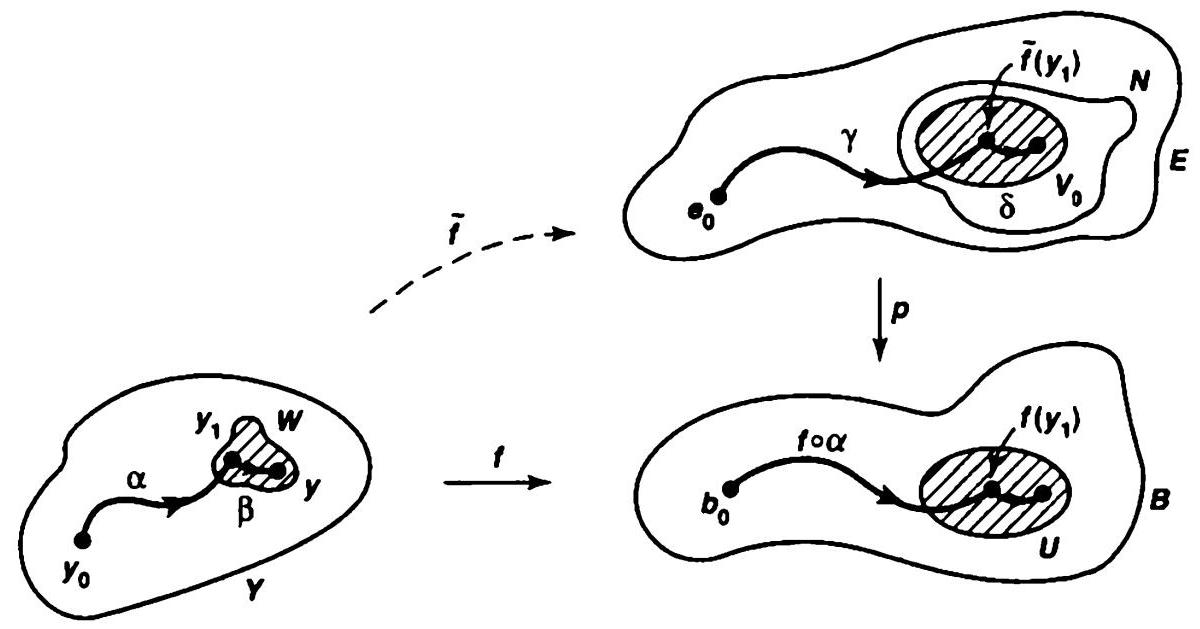
\includegraphics[width=1.0\textwidth]{images/79.1.jpg}
\end{center}
\hspace*{3em} 

Figure 79.1

To prove continuity of \(\widetilde{f}\) at the point \({y}_{1}\) of \(Y\) , we show that, given a neighborhood \(N\) of \(\widetilde{f}\left( {y}_{1}\right)\) , there is a neighborhood \(W\) of \({y}_{1}\) such that \(\widetilde{f}\left( W\right)  \subset  N\) . To begin, choose a path-connected neighborhood \(U\) of \(f\left( {y}_{1}\right)\) that is evenly covered by \(p\) . Break \({p}^{-1}\left( U\right)\) up into slices, and let \({V}_{0}\) be the slice that contains the point \(\widetilde{f}\left( {y}_{1}\right)\) . Replacing \(U\) by a smaller neighborhood of \(f\left( {y}_{1}\right)\) if necessary, we can assume that \({V}_{0} \subset  N\) . Let \({p}_{0} : {V}_{0} \rightarrow  U\) be obtained by restricting \(p\) ; then \({p}_{0}\) is a homeomorphism. Because \(f\) is continuous at \({y}_{1}\) and \(Y\) is locally path connected, we can find a path-connected neighborhood \(W\) of \({y}_{1}\) such that \(f\left( W\right)  \subset  U\) . We shall show that \(\widetilde{f}\left( W\right)  \subset  {V}_{0}\) ; then our result is proved.

Given \(y \in  W\) , choose a path \(\beta\) in \(W\) from \({y}_{1}\) to \(y\) . Since \(\widetilde{f}\) is well defined, \(\widetilde{f}\left( y\right)\) can be obtained by taking the path \(\alpha  * \beta\) from \({y}_{0}\) to \(y\) , lifting the path \(f \circ  \left( {\alpha  * \beta }\right)\) to a path in \(E\) beginning at \({e}_{0}\) , and letting \(\widetilde{f}\left( y\right)\) be the end point of this lifted path. Now \(\gamma\) is a lifting of \(\alpha\) that begins at \({e}_{0}\) . Since the path \(f \circ  \beta\) lies in \(U\) , the path \(\delta  = {p}_{0}^{-1} \circ  f \circ  \beta\) is a lifting of it that begins at \(\widetilde{f}\left( {y}_{1}\right)\) . Then \(\gamma  * \delta\) is a lifting of \(f \circ  \left( {\alpha  * \beta }\right)\) that begins at \({e}_{0}\) ; it ends at the point \(\delta \left( 1\right)\) of \({V}_{0}\) . Hence \(\bar{f}\left( W\right)  \subset  {V}_{0}\) , as desired.

Finally, we show \(\bar{f}\) is well defined. Let \(\alpha\) and \(\beta\) be two paths in \(Y\) from \({y}_{0}\) to \({y}_{1}\) . We must show that if we lift \(f \circ  \alpha\) and \(f \circ  \beta\) to paths in \(E\) beginning at \({e}_{0}\) , then these lifted paths end at the same point of \(E\) .

First, we lift \(f \circ  \alpha\) to a path \(\gamma\) in \(E\) beginning at \({e}_{0}\) ; then we lift \(f \circ  \bar{\beta }\) to a path \(\delta\) in \(E\) beginning at the end point \(\gamma \left( 1\right)\) of \(\gamma\) . Then \(\gamma  * \delta\) is a lifting of the loop \(f \circ  \left( {\alpha  * \bar{\beta }}\right)\) . Now by hypothesis,

\[
{f}_{ * }\left( {{\pi }_{1}\left( {Y,{y}_{0}}\right) }\right)  \subset  {p}_{ * }\left( {{\pi }_{1}\left( {E,{e}_{0}}\right) }\right) .
\]

Hence \(\left\lbrack  {f \circ  \left( {\alpha  * \bar{\beta }}\right) }\right\rbrack\) belongs to the image of \({p}_{ * }\) . Theorem 54.6 now implies that its lift \(\gamma  * \delta\) is a loop in \(E\) .

It follows that \(\bar{f}\) is well defined. For \(\bar{\delta }\) is a lifting of \(f \circ  \beta\) that begins at \({e}_{0}\) , and \(\gamma\) is a lifting of \(f \circ  \alpha\) that begins at \({e}_{0}\) , and both liftings end at the same point of \(E\) .
\end{proof}
\begin{theorem}
	Let \(p : E \rightarrow  B\) and \({p}^{\prime } : {E}^{\prime } \rightarrow  B\) be covering maps; let \(p\left( {e}_{0}\right)  =\)  \({p}^{\prime }\left( {e}_{0}^{\prime }\right)  = {b}_{0}\) . There is an equivalence \(h : E \rightarrow  {E}^{\prime }\) such that \(h\left( {e}_{0}\right)  = {e}_{0}^{\prime }\) if and only if the groups

\[
{H}_{0} = {p}_{ * }\left( {{\pi }_{1}\left( {E,{e}_{0}}\right) }\right) \;\text{ and }\;{H}_{0}^{\prime } = {p}_{ * }^{\prime }\left( {{\pi }_{1}\left( {{E}^{\prime },{e}_{0}^{\prime }}\right) }\right)
\]

are equal. If \(h\) exists, it is unique.
\end{theorem}

\begin{proof}
	We prove the ``only if'' part of the theorem. Given \(h\) , the fact that \(h\) is a homeomorphism implies that
\[
{h}_{ * }\left( {{\pi }_{1}\left( {E,{e}_{0}}\right) }\right)  = {\pi }_{1}\left( {{E}^{\prime },{e}_{0}^{\prime }}\right) .
\]

Since \({p}^{\prime } \circ  h = p\) , we have \({H}_{0} = {H}_{0}^{\prime }\) .

Now we prove the ``if'' part of the theorem; we assume that \({H}_{0} = {H}_{0}^{\prime }\) and show that \(h\) exists. We shall apply the preceding lemma (four times!). Consider the maps

\begin{center}
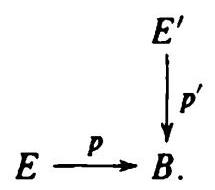
\includegraphics[width=0.2\textwidth]{images/79.11.jpg}
\end{center}
\hspace*{3em} 

Because \({p}^{\prime }\) is a covering map and \(E\) is path connected and locally path connected, there exists a map \(h : E \rightarrow  {E}^{\prime }\) with \(h\left( {e}_{0}\right)  = {e}_{0}^{\prime }\) that is a lifting of \(p\) (that is, such that \(\left. {{p}^{\prime } \circ  h = p}\right)\) . Reversing the roles of \(E\) and \({E}^{\prime }\) in this argument, we see there is a map \(k : {E}^{\prime } \rightarrow  E\) with \(k\left( {e}_{0}^{\prime }\right)  = {e}_{0}\) such that \(p \circ  k = {p}^{\prime }\) . Now consider the maps The map \(k \circ  h : E \rightarrow  E\) is a lifting of \(p\) (since \(p \circ  k \circ  h = {p}^{\prime } \circ  h = p\) ), with \(p\left( {e}_{0}\right)  = {e}_{0}\) . The identity map \({i}_{E}\) of \(E\) is another such lifting. The uniqueness part of the preceding lemma implies that \(k \circ  h = {i}_{E}\) . A similar argument shows that \(h \circ  k\) equals the identity map of \({E}^{\prime }\) .

\begin{center}
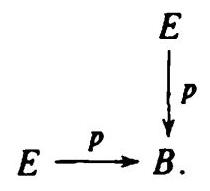
\includegraphics[width=0.2\textwidth]{images/79.12.jpg}
\end{center}
\hspace*{3em} 

We seem to have solved our equivalence problem. But there is a somewhat subtle point we have overlooked. We have obtained a necessary and sufficient condition for there to exist an equivalence \(h \cdot  E \rightarrow  {E}^{\prime }\) that carries the point \({e}_{0}\) to the point \({e}_{0}^{\prime }\) . But we have not yet determined under what conditions there exists an equivalence in general. It is possible that there may be no equivalence carrying \({e}_{0}\) to \({e}_{0}^{\prime }\) but that there is an equivalence carrying \({e}_{0}\) to some other point \({e}_{1}^{\prime }\) of \({\left( {p}^{\prime }\right) }^{-1}\left( {b}_{0}\right)\) . Can we determine whether this is the case merely by examining the subgroups \({H}_{0}\) and \({H}_{0}^{\prime }\) ? We consider this problem now.

If \({H}_{1}\) and \({H}_{2}\) are subgroups of a group \(G\) , you may recall from algebra that they are said to be \index{Conjugate subgroups}conjugate subgroups if \({H}_{2} = \alpha  \cdot  {H}_{1} \cdot  {\alpha }^{-1}\) for some element \(\alpha\) of \(G\) . Said differently, they are conjugate if the isomorphism of \(G\) with itself that maps \(x\) to \(\alpha  \cdot  x \cdot  {\alpha }^{-1}\) carries the group \({H}_{1}\) onto the group \({H}_{2}\) . It is easy to check that conjugacy is an equivalence relation on the collection of subgroups of \(G\) . The equivalence class of the subgroup \(H\) is called the \index{Conjugacy class}conjugacy class of \(H\) .
\end{proof}
\begin{lemma}
	Let \(p : E \rightarrow  B\) be a covering map. Let \({e}_{0}\) and \({e}_{1}\) be points of \({p}^{-1}\left( {b}_{0}\right)\) , and let \({H}_{i} = {p}_{ * }\left( {{\pi }_{1}\left( {E,{e}_{i}}\right) }\right)\) .
\end{lemma}

(a) If \(\gamma\) is a path in \(E\) from \({e}_{0}\) to \({e}_{1}\) , and \(\alpha\) is the loop \(p \circ  \gamma\) in \(B\) , then the equation \(\left\lbrack  \alpha \right\rbrack * {H}_{1} * {\left\lbrack  \alpha \right\rbrack  }^{-1} = {H}_{0}\) holds; hence \({H}_{0}\) and \({H}_{1}\) are conjugate.

(b) Conversely, given \({e}_{0}\) , and given a subgroup \(H\) of \({\pi }_{1}\left( {B,{b}_{0}}\right)\) conjugate to \({H}_{0}\) , there exists a point \({e}_{1}\) of \({p}^{-1}\left( {b}_{0}\right)\) such that \({H}_{1} = H\) .

\begin{proof}
	(a) First, we show that \(\left\lbrack  \alpha \right\rbrack * {H}_{1} * {\left\lbrack  \alpha \right\rbrack  }^{-1} \subset  {H}_{0}\) . Given an element \(\left\lbrack  h\right\rbrack\) of \({H}_{1}\) , we have \(\left\lbrack  h\right\rbrack = {p}_{ * }\left( \left\lbrack  \widetilde{h}\right\rbrack  \right)\) for some loop \(\widetilde{h}\) in \(E\) based at \({e}_{1}\) . Let \(\widetilde{k}\) be the path \(\widetilde{k} = \left( {\gamma  * \widetilde{h}}\right)  * \widetilde{\gamma }\) ; it is a loop in \(E\) based at \({e}_{0}\) , and
\[
{p}_{ * }\left( \left\lbrack  \bar{k}\right\rbrack  \right)  = \left\lbrack  {\left( {\alpha  * h}\right)  * \bar{\alpha }}\right\rbrack = \left\lbrack  \alpha \right\rbrack * \left\lbrack  h\right\rbrack * {\left\lbrack  \alpha \right\rbrack  }^{-1},
\]

so the latter element belongs to \({p}_{ * }\left( {{\pi }_{1}\left( {E,{e}_{0}}\right) }\right)  = {H}_{0}\) , as desired. See Figure 79.2.

Now we show that \(\left\lbrack  \alpha \right\rbrack * {H}_{1} * {\left\lbrack  \alpha \right\rbrack  }^{-1} \supset  {H}_{0}\) . Note that \(\bar{\gamma }\) is a path from \({e}_{1}\) to \({e}_{0}\) and \(\bar{\alpha }\) equals the loop \(p \circ  \bar{\gamma }\) . By the result just proved, we have

\[
\left\lbrack  \bar{\alpha }\right\rbrack * {H}_{0} * {\left\lbrack  \bar{\alpha }\right\rbrack  }^{-1} \subset  {H}_{1}
\]

which implies out desired result.

(b) To prove the converse, let \({e}_{0}\) be given and let \(H\) be conjugate to \({H}_{0}\) . Then \({H}_{0} = \left\lbrack  \alpha \right\rbrack * H * {\left\lbrack  \alpha \right\rbrack  }^{-1}\) for some loop \(\alpha\) in \(B\) based at \({b}_{0}\) . Let \(\gamma\) be the lifting of \(\alpha\) to a path in \(E\) beginning at \({e}_{0}\) , and let \({e}_{1} = \gamma \left( 1\right)\) . Then (a) implies that \({H}_{0} = \left\lbrack  \alpha \right\rbrack * {H}_{1} * {\left\lbrack  \alpha \right\rbrack  }^{-1}\) . We conclude that \(H = {H}_{1}\) .

\begin{center}
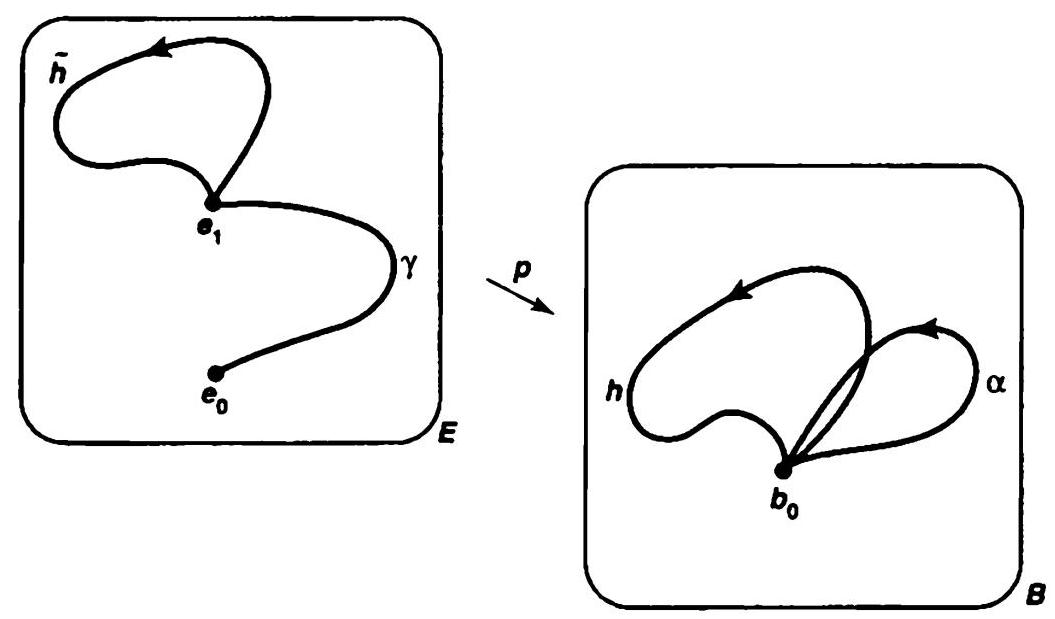
\includegraphics[width=0.9\textwidth]{images/79.2.jpg}
\end{center}
\hspace*{3em} 

Figure 79.2
\end{proof}
\begin{theorem}
	Let \(p : E \rightarrow  B\) and \({p}^{\prime } : {E}^{\prime } \rightarrow  B\) be covering maps; let \(p\left( {e}_{0}\right)  =\)  \({p}^{\prime }\left( {e}_{0}^{\prime }\right)  = {b}_{0}\) . The covering maps \(p\) and \({p}^{\prime }\) are equivalent if and only if the subgroups

\[
{H}_{0} = {p}_{ * }\left( {{\pi }_{1}\left( {E,{e}_{0}}\right) }\right) \;\text{ and }\;{H}_{0}^{\prime } = {p}_{ * }^{\prime }\left( {{\pi }_{1}\left( {{E}^{\prime },{e}_{0}^{\prime }}\right) }\right)
\]

of \({\pi }_{1}\left( {B,{b}_{0}}\right)\) are conjugate.
\end{theorem}

\begin{proof}
	If \(h : E \rightarrow  {E}^{\prime }\) is an equivalence, let \({e}_{1}^{\prime } = h\left( {e}_{0}\right)\) , and let \({H}_{1}^{\prime } = {p}_{ * }\left( {{\pi }_{1}\left( {{E}^{\prime },{e}_{1}^{\prime }}\right) }\right)\) Theorem 79.2 implies that \({H}_{0} = {H}_{1}^{\prime }\) , while the preceding lemma tells us that \({H}_{1}^{\prime }\) is conjugate to \({H}_{0}^{\prime }\) .
Conversely, if the groups \({H}_{0}\) and \({H}_{0}^{\prime }\) are conjugate, the preceding lemma implies there is a point \({e}_{1}^{\prime }\) of \({E}^{\prime }\) such that \({H}_{1}^{\prime } = {H}_{0}\) . Theorem 79.2 then gives us an equivalence \(h : E \rightarrow  {E}^{\prime }\) such that \(h\left( {e}_{0}\right)  = {e}_{1}^{\prime }\) .

\begin{centeredblock}
\begin{example}
	Consider covering spaces of the circle \(B = {S}^{1}\) . Because \({\pi }_{1}\left( {B,{b}_{0}}\right)\) is abelian, two subgroups of \({\pi }_{1}\left( {B,{b}_{0}}\right)\) are conjugate if and only if they are equal. Therefore two coverings of \(B\) are equivalent if and only if they correspond to the same subgroup of \({\pi }_{1}\left( {B,{b}_{0}}\right)\) .

Now \({\pi }_{1}\left( {B,{b}_{0}}\right)\) is isomorphic to the integers \(\mathbb{Z}\) . What are the subgroups of \({\mathbb{Z}}^{2}\) It is standard theorem of modern algebra that, given a nontrivial subgroup of \(\mathbb{Z}\) , it must be the group \({G}_{n}\) consisting of all multiples of \(n\) , for some \(n \in  {\mathbb{Z}}_{ + }\) .

We have studied one covering space of the circle, the covering \(p : \mathbb{R} \rightarrow  {S}^{1}\) It must correspond to the trivial subgroup of \({\pi }_{1}\left( {{S}^{1},{b}_{0}}\right)\) , because \(\mathbb{R}\) is simply connected We have also considered the covering \(p : {S}^{1} \rightarrow  {S}^{1}\) defined by \(p\left( z\right)  = {z}^{n}\) , where \(z\) is a complex number. In this case, the map \({p}_{ * }\) carries a generator of \({\pi }_{1}\left( {{S}^{1},{b}_{0}}\right)\) into \(n\) times itself. Therefore, the group \({p}_{ * }\left( {{\pi }_{1}\left( {{S}^{1},{b}_{0}}\right) }\right)\) corresponds to the subgroup \({G}_{n}\) of \(\mathbb{Z}\) under the standard isomorphism of \({\pi }_{1}\left( {{S}^{1},{b}_{0}}\right)\) with \(\mathbb{Z}\) .

We conclude from the preceding theorem that every path-connected covering space of \({S}^{1}\) is equivalent to one of these coverings.
\end{example}
\end{centeredblock}
\end{proof}
\section*{Exercises}
\begin{enumerate}[itemsep=0.4em, parsep=0pt, topsep=0pt, partopsep=0pt, leftmargin=*, label=\arabic*., ref=\arabic*]
\item Show that if \(n > 1\) , every continuous map \(f : {S}^{n} \rightarrow  {S}^{1}\) is nulhomotopic. [Hint: Use the lifting lemma.]
\item
  \begin{enumerate}[itemsep=0.2em, parsep=0pt, topsep=0pt, partopsep=0pt, leftmargin=*, label=(\alph*), align=left]
  \item Show that every continuous map \(f : {P}^{2} \rightarrow  {S}^{1}\) is nulhomotopic.

  \item Find a continuous map of the torus into \({S}^{1}\) that is not nulhomotopic.
  \end{enumerate}
\item Let \(p : E \rightarrow  B\) be a covering map; let \(p\left( {e}_{0}\right)  = {b}_{0}\) . Show that \({H}_{0} =\)  \({p}_{ * }\left( {{\pi }_{1}\left( {E,{e}_{0}}\right) }\right)\) is a normal subgroup of \({\pi }_{1}\left( {B,{b}_{0}}\right)\) if and only if for every pair of points \({e}_{1},{e}_{2}\) of \({p}^{-1}\left( {b}_{0}\right)\) , there is an equivalence \(h : E \rightarrow  E\) with \(h\left( {e}_{1}\right)  = {e}_{2}\) .
\item Let \(T = {S}^{1} \times  {S}^{1}\) , the torus. There is an isomorphism of \({\pi }_{1}\left( {T,{b}_{0} \times  {b}_{0}}\right)\) with \(\mathbb{Z} \times  \mathbb{Z}\) induced by projections of \(T\) onto its two factors.
  \begin{enumerate}[itemsep=0.2em, parsep=0pt, topsep=0pt, partopsep=0pt, leftmargin=*, label=(\alph*), align=left]
  \item Find a covering space of \(T\) corresponding to the subgroup of \(\mathbb{Z} \times  \mathbb{Z}\) generated by the element \(m \times  0\) , where \(m\) is a positive integer.
  \item Find a covering space of \(T\) corresponding to the trivial subgroup of \(\mathbb{Z} \times  \mathbb{Z}\) .
  \item Find a covering space of \(T\) corresponding to the subgroup of \(\mathbb{Z} \times  \mathbb{Z}\) generated by \(m \times  0\) and \(0 \times  n\) , where \(m\) and \(n\) are positive integers. *5. Let \(T = {S}^{1} \times  {S}^{1}\) be the torus; let \({x}_{0} = {b}_{0} \times  {b}_{0}\) .
  \item Prove the following: \textsl{Theorem.} Every isomorphism of \({\pi }_{1}\left( {T,{x}_{0}}\right)\) with itself is induced by a homeomorphism of \(T\) with itself that maps \({x}_{0}\) to \({x}_{0}\) .  [Hint: Let \(p : {\mathbb{R}}^{2} \rightarrow  T\) be the usual covering map. If \(A\) is a \(2 \times  2\) matrix with integer entries, the linear map \({T}_{A} : {\mathbb{R}}^{2} \rightarrow  {\mathbb{R}}^{2}\) with matrix \(A\) induces a continuous map \(f : T \rightarrow  T\) . Furthermore, \(f\) is a homeomorphism if \(A\) is invertible over the integers.]
  \item Prove the following: \textsl{Theorem.} If \(E\) is a covering space of \(T\) , then \(E\) is homeomorphic either to \({\mathbb{R}}^{2}\) , or to \({S}^{1} \times  \mathbb{R}\) , or to \(T\) .  [Hint: You may use the following result from algebra: If \(F\) is a free abelian group of rank 2 and \(N\) is a nontrivial subgroup, then there is a basis \({a}_{1},{a}_{2}\) for \(F\) such that either (1) \(m{a}_{1}\) is a basis for \(N\) , for some positive integer \(m\) , or \(\left( 2\right) m{a}_{1},n{a}_{2}\) is a basis for \(N\) , where \(m\) and \(n\) are positive integers.] *6. Prove the following: \textsl{Theorem.} Let \(G\) be a topological group with multiplication operation \(m : G \times\)  \(G \rightarrow  G\) and identity element \(e\) . Assume \(p : \bar{G} \rightarrow  G\) is a covering map. Given \(\widetilde{e}\) with \(p\left( \widetilde{e}\right)  = e\) , there is a unique multiplication operation on \(\bar{G}\) that makes it into a topological group such that \(\widetilde{e}\) is the identity element and \(p\) is a homomorphism.  Proof. Recall that, by our convention, \(G\) and \(\widetilde{G}\) are path connected and locally path connected.
  \item Let \(I : G \rightarrow  G\) be the map \(I\left( g\right)  = {g}^{-1}\) . Show there exist unique maps \(\bar{m} : \widetilde{G} \times  \widetilde{G} \rightarrow  \widetilde{G}\) and \(\widetilde{I} : \widetilde{G} \rightarrow  \widetilde{G}\) with \(\widetilde{m}\left( {\widetilde{e} \times  \widetilde{e}}\right)  = \widetilde{e}\) and \(\widetilde{I}\left( \bar{e}\right)  = \bar{e}\) such that \(p \circ  \widetilde{m} = m \circ  \left( {p \times  p}\right)\) and \(p \circ  \widetilde{I} = I \circ  p\) .
  \item Show the maps \(\widetilde{G} \rightarrow  \widetilde{G}\) given by \(\widetilde{g} \rightarrow  \widetilde{m}\left( {\widetilde{e} \times  \widetilde{g}}\right)\) and \(\widetilde{g} \rightarrow  \widetilde{m}\left( {\widetilde{g} \times  \widetilde{e}}\right)\) equal the identity map of \(\widetilde{G}\) . [Hint: Use the uniqueness part of Lemma 79.1.]
  \item Show the maps \(\widetilde{G} \rightarrow  \widetilde{G}\) given by \(\widetilde{g} \rightarrow  \widetilde{m}\left( {\widetilde{g} \times  \widetilde{I}\left( \widetilde{g}\right) }\right)\) and \(\widetilde{g} \rightarrow  \widetilde{m}\left( {\widetilde{I}\left( \widetilde{g}\right)  \times  \widetilde{g}}\right)\) map \(\widetilde{G}\) to \(\widetilde{e}\) .
  \item Show the maps \(\bar{G} \times  \widetilde{G} \times  \bar{G} \rightarrow  \bar{G}\) given by \[ \begin{aligned}  & \widetilde{g} \times  {\widetilde{g}}^{\prime } \times  {\widetilde{g}}^{\prime \prime } \rightarrow  \widetilde{m}\left( {\widetilde{g} \times  \bar{m}\left( {{\widetilde{g}}^{\prime } \times  {\widetilde{g}}^{\prime \prime }}\right) }\right) \\  & \widetilde{g} \times  {\widetilde{g}}^{\prime } \times  {\widetilde{g}}^{\prime \prime } \rightarrow  \bar{m}\left( {\widetilde{m}\left( {\widetilde{g} \times  {\widetilde{g}}^{\prime }}\right)  \times  {\widetilde{g}}^{\prime \prime }}\right) \end{aligned} \] are equal.
  \item Complete the proof.
  \end{enumerate}
\item Let \(p : \widetilde{G} \rightarrow  G\) be a homomorphism of topological groups that is a covering map. Show that if \(G\) is abelian, so is \(\bar{G}\) .
\end{enumerate}
\section*{§ 80 The Universal Covering Space}

Suppose \(p : E \rightarrow  B\) is a covering map, with \(p\left( {e}_{0}\right)  = {b}_{0}\) . If \(E\) is simply connected, then \(E\) is called a \index{Universal covering space}universal covering space of \(B\) . Since \({\pi }_{1}\left( {E,{e}_{0}}\right)\) is trivial, this covering space corresponds to the trivial subgroup of \({\pi }_{1}\left( {B,{b}_{0}}\right)\) under the correspondence defined in the preceding section. Theorem 79.4 thus implies that any two universal covering spaces of \(B\) are equivalent. For this reason, we often speak of ``the'' universal covering space of a given space \(B\) . Not every space has a universal covering space, as we shall see. For the moment, we shall simply assume that B has a universal covering space and derive some consequences of this assumption.

We prove two preliminary lemmas:

\begin{lemma}
	Let \(B\) be path connected and locally path connected. Let \(p : E \rightarrow  B\) be a covering map in the former sense (so that \(E\) is not required to be path connected). If \({E}_{0}\) is a path component of \(E\) , then the map \({p}_{0} : {E}_{0} \rightarrow  B\) obtained by restricting \(p\) is a covenng map.
\end{lemma}

\begin{proof}
	We first show \({p}_{0}\) is surjective. Since the space \(E\) is locally homeomorphic to \(B\) , it is locally path connected. Therefore \({E}_{0}\) is open in \(E\) . It follows that \(p\left( {E}_{0}\right)\) is open in \(B\) . We show that \(p\left( {E}_{0}\right)\) is also closed in \(B\) , so that \(p\left( {E}_{0}\right)  = B\) .
Let \(x\) be a point of \(B\) beloriging to the closure of \(p\left( {E}_{0}\right)\) . Let \(U\) be a path-connected neighborhood of \(x\) that is evenly covered by \(p\) . Since \(U\) contains a point of \(p\left( {E}_{0}\right)\) , some slice \({V}_{\alpha }\) of \({p}^{-1}\left( U\right)\) must intersect \({E}_{0}\) . Since \({V}_{\alpha }\) is homeomorphic to \(U\) , it is path connected; therefore it must be contained in \({E}_{0}\) . Then \(p\left( {V}_{\alpha }\right)  = U\) is contained in \(p\left( {E}_{0}\right)\) , so that in particular, \(x \in  p\left( {E}_{0}\right)\) .

Now we show \({p}_{0} : {E}_{0} \rightarrow  B\) is a covering map. Given \(x \in  B\) , choose a neighborhood \(U\) of \(x\) as before. If \({V}_{\alpha }\) is a slice of \({p}^{-1}\left( U\right)\) , then \({V}_{\alpha }\) is path connected; if it intersects \({E}_{0}\) , it lies in \({E}_{0}\) . Therefore, \({p}_{0}^{-1}\left( U\right)\) equals the union of those slices \({V}_{\alpha }\) of \({p}^{-1}\left( U\right)\) that intersect \({E}_{0}\) ; each of these is open in \({E}_{0}\) and is mapped homeomorphi-cally by \({p}_{0}\) onto \(U\) . Thus \(U\) is evenly covered by \({p}_{0}\) .
\end{proof}
\begin{lemma}
	Let \(p,q\) , and \(r\) be continuous maps with \(p = r \circ  q\) , as in the following diagram:

\begin{center}
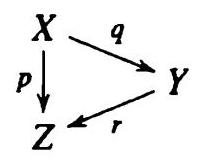
\includegraphics[width=0.2\textwidth]{images/80.01.jpg}
\end{center}
\hspace*{3em} 

(a) If \(p\) and \(q\) are covering maps, so is \(q\) .

*(b) If \(p\) and \(q\) are covering maps, so is \(r\) .
\end{lemma}

\begin{proof}
	By our convention, \(X,Y\) , and \(Z\) are path connected and locally path connected. Let \({x}_{0} \in  X\) ; set \({y}_{0} = q\left( {x}_{0}\right)\) and \({z}_{0} = p\left( {x}_{0}\right)\) .
(a) Assume that \(p\) and \(r\) are covering maps. We show first that \(q\) is surjective. Given \(y \in  Y\) , choose a path \(\bar{\alpha }\) in \(Y\) from \({y}_{0}\) to \(y\) . Then \(\alpha  = r \circ  \bar{\alpha }\) is a path in \(Z\) beginning at \({z}_{0}\) ; let \(\widetilde{\bar{\alpha }}\) be a lifting of \(\alpha\) to a path in \(X\) beginning at \({x}_{0}\) . Then \(q \circ  \widetilde{\bar{\alpha }}\) is a lifting of \(\alpha\) to \(Y\) that begins at \({y}_{0}\) . By uniqueness of path liftings, \(\widetilde{\alpha } = q \circ  \widetilde{\bar{\alpha }}\) . Then \(q\) maps the end point of \(\overline{\bar{\alpha }}\) to the end point \(y\) of \(\bar{\alpha }\) . Thus \(q\) is surjective.

Given \(y \in  Y\) , we find a neighborhood of \(y\) that is evenly covered by \(q\) . Let \(z =\)  \(r\left( y\right)\) . Since \(p\) and \(r\) are covering maps, we can find a path-connected neighborhood \(U\) of \(z\) that is evenly covered by both \(p\) and \(r\) . Let \(V\) be the slice of \({r}^{-1}\left( U\right)\) that contains the point \(y\) ; we show \(V\) is evenly covered by \(q\) . Let \(\left\{  {U}_{\alpha }\right\}\) be the collection of slices of \({p}^{-1}\left( U\right)\) . Now \(q\) maps each set \({U}_{\alpha }\) into the set \({r}^{-1}\left( U\right)\) ; because \({U}_{\alpha }\) is connected, it must be mapped by \(q\) into a single one of the slices of \({r}^{-1}\left( U\right)\) . Therefore, \({q}^{-1}\left( V\right)\) equals the union of those slices \({U}_{\alpha }\) that are mapped by \(q\) into \(V\) . It is easy to see that each such \({U}_{\alpha }\) is mapped homeomorphically onto \(V\) by \(q\) . For let \({p}_{0},{q}_{0},{r}_{0}\) be the maps obtained by restricting \(p,q\) , and \(r\) , respectively, as indicated in the following diagram:

\begin{center}
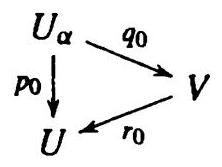
\includegraphics[width=0.2\textwidth]{images/80.02.jpg}
\end{center}
\hspace*{3em} 

Because \({p}_{0}\) and \({r}_{0}\) are homeomorphisms, so is \({q}_{0} = {r}_{0}^{-1} \circ  {p}_{0}\) .

*(b) We shall use this result only in the exercises. Assume that \(p\) and \(q\) are covering maps. Because \(p = r \circ  q\) and \(p\) is surjective, \(r\) is also surjective.

Given \(z \in  Z\) , let \(U\) be a path-connected neighborhood of \(z\) that is evenly covered by \(p\) . We show that \(U\) is also evenly covered by \(r\) . Let \(\left\{  {V}_{\beta }\right\}\) be the collection of path components of \({r}^{-1}\left( U\right)\) ; these sets are disjoint and open in \(Y\) . We show that for each \(\beta\) , the map \(r\) carries \({V}_{\beta }\) homeomorphically onto \(U\) .

Let \(\left\{  {U}_{\alpha }\right\}\) be the collection of slices of \({p}^{-1}\left( U\right)\) ; they are disjoint, open, and path connected, so they are the path components of \({p}^{-1}\left( U\right)\) . Now \(q\) maps each \({U}_{\alpha }\) into the set \({r}^{-1}\left( U\right)\) ; because \({U}_{\alpha }\) is connected, it must be mapped by \(q\) into one of the sets \({V}_{\beta }\) . Therefore \({q}^{-1}\left( {V}_{\beta }\right)\) equals the union of a subcollection of the collection \(\left\{  {U}_{\alpha }\right\}\) . Theorem 53.2 and Lemma 80.1 together imply that if \({U}_{{\alpha }_{0}}\) is any one of the path components of \({q}^{-1}\left( {V}_{\beta }\right)\) then the map \({q}_{0} : {U}_{{\alpha }_{0}} \rightarrow  {V}_{\beta }\) obtained by restricting \(q\) is a covering map. In particular, \({q}_{0}\) is surjective. Hence \({q}_{0}\) is a homeomorphism, being continuous, open, and injective as well. Consider the maps

\begin{center}
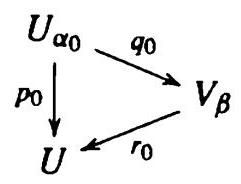
\includegraphics[width=0.2\textwidth]{images/80.03.jpg}
\end{center}
\hspace*{3em} 

obtained by restricting \(p,q\) , and \(r\) . Because \({p}_{0}\) and \({q}_{0}\) are homeomorphisms, so is \({r}_{0}\) .
\end{proof}
\begin{theorem}
	Let \(p : E \rightarrow  B\) be a covering map, with \(E\) simply connected. Given any covering map \(r : Y \rightarrow  B\) , there is a covering map \(q : E \rightarrow  Y\) such that \(r \circ  q = p\) .
\end{theorem}

\begin{center}
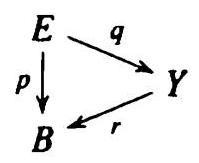
\includegraphics[width=0.2\textwidth]{images/80.04.jpg}
\end{center}
\hspace*{3em} 

This theorem shows why \(E\) is called a universal covering space of \(B\) ; it covers every other covering space of \(B\) .

\begin{proof}
	Let \({b}_{0} \in  B\) ; choose \({e}_{0}\) and \({y}_{0}\) so that \(p\left( {e}_{0}\right)  = {b}_{0}\) and \(r\left( {y}_{0}\right)  = {b}_{0}\) . We apply Lemma 79.1 to construct \(q\) . The map \(r\) is a covering map, and the condition
\[
{p}_{ * }\left( {{\pi }_{1}\left( {E,{e}_{0}}\right) }\right)  \subset  {r}_{ * }\left( {{\pi }_{1}\left( {Y,{y}_{0}}\right) }\right)
\]

is satisfied trivially because \(E\) is simply connected. Therefore, there is a map \(q : E \rightarrow\)  \(Y\) such that \(r \circ  q = p\) and \(q\left( {e}_{0}\right)  = {y}_{0}\) . It follows from the preceding lemma that \(q\) is a covering map.

Now we give an example of a space that has no universal covering space. We need the following lemma.
\end{proof}
\begin{lemma}
	Let \(p : E \rightarrow  B\) be a covering map; let \(p\left( {e}_{0}\right)  = {b}_{0}\) . If \(E\) is simply connected, then \({b}_{0}\) has a neighborhood \(U\) such that inclusion \(i : U \rightarrow  B\) induces the trivial homomorphism

\[
{i}_{ * } : {\pi }_{1}\left( {U,{b}_{0}}\right)  \rightarrow  {\pi }_{1}\left( {B,{b}_{0}}\right) .
\]
\end{lemma}

\begin{proof}
	Let \(U\) be a neighborhood of \({b}_{0}\) that is evenly covered by \(p\) ; break \({p}^{-1}\left( U\right)\) up into slices; let \({U}_{\alpha }\) be the slice containing \({e}_{0}\) . Let \(f\) be a loop in \(U\) based at \({b}_{0}\) . Because \(p\) defines a homeomorphism of \({U}_{\alpha }\) with \(U\) , the loop \(f\) lifts to a loop \(\widetilde{f}\) in \({U}_{\alpha }\) based at \({e}_{0}\) . Since \(E\) is simply connected, there is a path homotopy \(\widetilde{F}\) in \(E\) between \(\widetilde{f}\) and a constant loop. Then \(p \circ  \widetilde{F}\) is a path homotopy in \(B\) between \(f\) and a constant loop.
\begin{centeredblock}
\begin{example}
	Let \(X\) be our familiar ``infinite earring'' in the plane, if \({C}_{n}\) is the circle of radius \(1/n\) in the plane with center at the point \(\left( {1/n,0}\right)\) , then \(X\) is the union of the curcles \({C}_{n}\) . Let \({b}_{0}\) be the origin; we show that if \(U\) is any neighborhood of \({b}_{0}\) in \(X\) , then the homomorphism of fundamental groups induced by inclusion \(i : U \rightarrow  X\) is not trivial.

Given \(n\) , there is a retr\index{fixed-point-free action@Fixed-point-free action}Fixed-point-free action action \(r : X \rightarrow  {C}_{n}\) obtained by lettung \(r\) map each circle \({C}_{t}\) for \(i \neq  n\) to the point \({b}_{0}\) . Choose \(n\) large enough that \({C}_{n}\) lies in \(U\) . Then in the following diagram of homomorphisms induced by inclusion, \({j}_{ * }\) is injective, hence \({i}_{ * }\) cannot be trivial.

\begin{center}
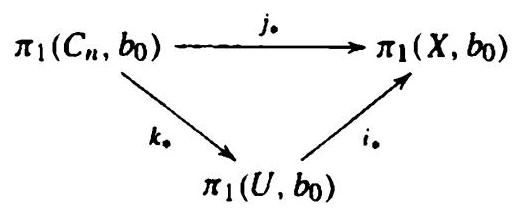
\includegraphics[width=0.4\textwidth]{images/80.05.jpg}
\end{center}
\hspace*{3em}

It follows that even though \(X\) is path connected and locally path connected, it has no universal covering space.
\end{example}
\end{centeredblock}
\end{proof}
\section*{Exercise}

1. Let \(q : X \rightarrow  Y\) and \(r : Y \rightarrow  Z\) be maps; let \(p = r \circ  q\) .

(a) Let \(q\) and \(r\) be covering maps. Show that if \(Z\) has a universal covering space, then \(p\) is a covering map. Compare Exercise 4 of  \S 53.

*(b) Give an example where \(q\) and \(r\) are covering maps but \(p\) is not.

\section*{*§  81 Covering Transformations}

Given a covering map \(p : E \rightarrow  B\) , it is of some interest to consider the set of all equivalences of this covering space with itself. Such an equivalence is called a \index{Covering transformation}covering transformation. Composites and inverses of covering transformations are covering transformations, so this set forms a group; it is called the \index{Group of covering transformations}group of covering transformations and denoted \(\mathcal{C}\left( {E,p,B}\right)\) .

Throughout this section, we shall assume that \(p : E \rightarrow  B\) is a covering map with \(p\left( {e}_{0}\right)  = {b}_{0}\) ; and we shall let \({H}_{0} = {p}_{ * }\left( {{\pi }_{1}\left( {E,{e}_{0}}\right) }\right)\) . We shall show that the group \(\mathcal{C}\left( {E,p,B}\right)\) is completely determined by the group \({\pi }_{1}\left( {B,{b}_{0}}\right)\) and the subgroup \({H}_{0}\) . Specifically, we shall show that if \(N\left( {H}_{0}\right)\) is the largest subgroup of \({\pi }_{1}\left( {B,{b}_{0}}\right)\) of which \({H}_{0}\) is a normal subgroup, then \(\mathcal{C}\left( {E,p,B}\right)\) is isomorphic to \(N\left( {H}_{0}\right) /{H}_{0}\) .

We define \(N\left( {H}_{0}\right)\) formally as follows:

\begin{definition}
	If \(H\) is a subgroup of the group \(G\) , then the \index{Normalizer}normalizer of \(H\) in \(G\) is the subset of \(G\) defined by the equation

\[
N\left( H\right)  = \left\{  {g \mid  {gH}{g}^{-1} = H}\right\}  .
\]
\end{definition}

It is easy to see that \(N\left( H\right)\) is a subgroup of \(G\) . It follows from the definition that it contains \(H\) as a normal subgroup and is the largest such subgroup of \(G\) .

The correspondence between the groups \(N\left( {H}_{0}\right) /{H}_{0}\) and \(\mathcal{C}\left( {E,p,B}\right)\) is established by using the lifting correspondence of \( \S {54}\) and the results about the existence of equivalences proved in \( \S {79}\) . We make the following definition:

\begin{definition}
	Given \(p : E \rightarrow  B\) with \(p\left( {e}_{0}\right)  = {b}_{0}\) , let \(F\) be the set \(F = {p}^{-1}\left( {e}_{0}\right)\) . Let

\[
\Phi  : {\pi }_{1}\left( {B,{b}_{0}}\right) /{H}_{0} \rightarrow  F
\]

be the lifting correspondence of Theorem 54.6; it is a bijection. Define also a correspondence

\[
\Psi  : \mathcal{C}\left( {E,p,B}\right)  \rightarrow  F
\]

by setting \(\Psi \left( h\right)  = h\left( {e}_{0}\right)\) for each covering transformation \(h : E \rightarrow  E\) . Since \(h\) is uniquely determined once its value at \({e}_{0}\) is known, the correspondence \(\Psi\) is injective.
\end{definition}

\begin{lemma}
	The image of the map \(\Psi\) equals the image under \(\Phi\) of the subgroup \(N\left( {H}_{0}\right) /{H}_{0}\) of \({\pi }_{1}\left( {B,{b}_{0}}\right) /{H}_{0}\) .
\end{lemma}

\begin{proof}
	Recall that the lifting correspondence \(\phi  : {\pi }_{1}\left( {B,{b}_{0}}\right)  \rightarrow  F\) is defined as follows: Given a loop \(\alpha\) in \(B\) at \({b}_{0}\) , let \(\gamma\) be its lift to \(E\) beginning at \({e}_{0}\) ; let \({e}_{1} = \gamma \left( 1\right)\) ; and define \(\phi\) by setting \(\phi \left( \left\lbrack  \alpha \right\rbrack  \right)  = {e}_{1}\) . To prove the lemma, we need to show that there is a covering transformation \(h : E \rightarrow  E\) with \(h\left( {e}_{0}\right)  = {e}_{1}\) if and only if \(\left\lbrack  \alpha \right\rbrack \in  N\left( {H}_{0}\right)\) .
This is easy. Lemma 79.1 tells us that \(h\) exists if and only if \({H}_{0} = {H}_{1}\) , where \({H}_{1} = {p}_{ * }\left( {{\pi }_{1}\left( {E,{e}_{1}}\right) }\right)\) . And Lemma 79.3 tells us that \(\left\lbrack  \alpha \right\rbrack * {H}_{1} * {\left\lbrack  \alpha \right\rbrack  }^{-1} = {H}_{0}\) . Hence \(h\) exists if and only if \(\left\lbrack  \alpha \right\rbrack * {H}_{0} * {\left\lbrack  \alpha \right\rbrack  }^{-1} = {H}_{0}\) , which is simply the statement that \(\left\lbrack  \alpha \right\rbrack \in\)  \(N\left( {H}_{0}\right)\) .
\end{proof}
\begin{theorem}
	The bijection

\[
{\Phi }^{-1} \circ  \Psi  : \mathcal{C}\left( {E,p,B}\right)  \rightarrow  N\left( {H}_{0}\right) /{H}_{0}
\]

is an isomorphism of groups.
\end{theorem}

\begin{proof}
	We need only show that \({\Phi }^{-1} \circ  \Psi\) is a homomorphism. Let \(h,k : E \rightarrow  E\) be covering transformations. Let \(h\left( {e}_{0}\right)  = {e}_{1}\) and \(k\left( {e}_{0}\right)  = {e}_{2}\) ; then
\[
\Psi \left( h\right)  = {e}_{1}\;\text{ and }\;\Psi \left( k\right)  = {e}_{2},
\]

by definition. Choose paths \(\gamma\) and \(\delta\) in \(E\) from \({e}_{0}\) to \({e}_{1}\) and \({e}_{2}\) , respectively. If \(\alpha  = p \circ  \gamma\) and \(\beta  = p \circ  \delta\) , then

\[
\Phi \left( {\left\lbrack  \alpha \right\rbrack  {H}_{0}}\right)  = {e}_{1}\;\text{ and }\;\Phi \left( {\left\lbrack  \beta \right\rbrack  {H}_{0}}\right)  = {e}_{2},
\]

by definition. Let \({e}_{3} = h\left( {k\left( {e}_{0}\right) }\right)\) ; then \(\Psi \left( {h \circ  k}\right)  = {e}_{3}\) . We show that

\[
\Phi \left( {\left\lbrack  {\alpha  * \beta }\right\rbrack  {H}_{0}}\right)  = {e}_{3},
\]

and the proof is complete.

Since \(\delta\) is a path from \({e}_{0}\) to \({e}_{2}\) , the path \(h \circ  \delta\) is a path from \(h\left( {e}_{0}\right)  = {e}_{1}\) to \(h\left( {e}_{2}\right)  = h\left( {k\left( {e}_{0}\right) }\right)  = {e}_{3}\) . See Figure 81.1. Then the product \(\gamma  * \left( {h \circ  \delta }\right)\) is defined and is a path from \({e}_{0}\) to \({e}_{3}\) . It is a lifting of \(\alpha  * \beta\) , since \(p \circ  \gamma  = \alpha\) and \(p \circ  h \circ  \delta  = p \circ  \delta  = \beta\) . Therefore \(\Phi \left( {\left\lbrack  {\alpha  * \beta }\right\rbrack  {H}_{0}}\right)  = {e}_{3}\) , as desired.

\begin{center}
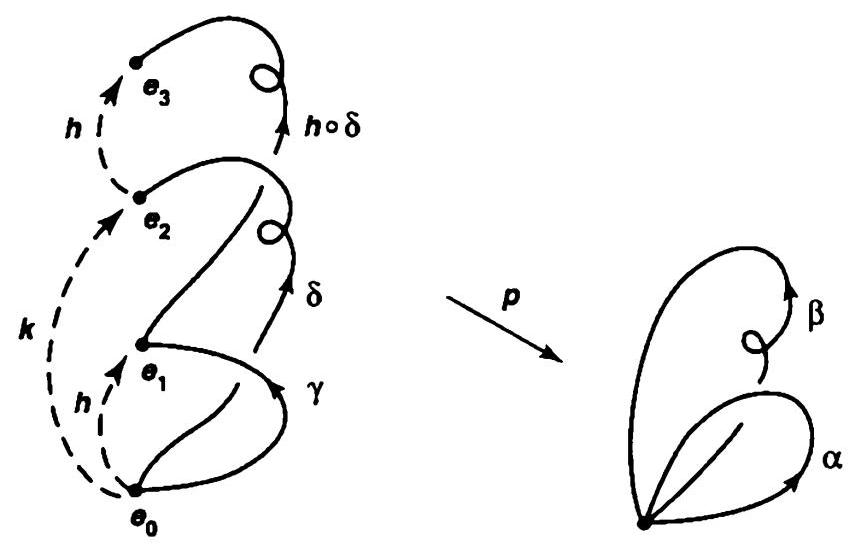
\includegraphics[width=0.7\textwidth]{images/81.1.jpg}
\end{center}
\hspace*{3em} 

Figure 81.1
\end{proof}
\begin{corollary}
	The group \({H}_{0}\) is a normal subgroup of \({\pi }_{1}\left( {B,{b}_{0}}\right)\) if and only if for every pair of points \({e}_{1}\) and \({e}_{2}\) of \({p}^{-1}\left( {b}_{0}\right)\) , there is a covering transformation \(h : E \rightarrow\)  \(E\) with \(h\left( {e}_{1}\right)  = {e}_{2}\) . In this case, there is an isomorphism

\[
{\Phi }^{-1} \circ  \Psi  : \mathcal{C}\left( {E,p,B}\right)  \rightarrow  {\pi }_{1}\left( {B,{b}_{0}}\right) /{H}_{0}.
\]
\end{corollary}

\begin{corollary}
	Let \(p : E \rightarrow  B\) be a covering map. If \(E\) is simply connected, then

\[
\mathcal{C}\left( {E,p,B}\right)  \cong  {\pi }_{1}\left( {B,{b}_{0}}\right) .
\]

If \({H}_{0}\) is a normal subgroup of \({\pi }_{1}\left( {B,{b}_{0}}\right)\) , then \(p : E \rightarrow  B\) is called a regular covering map (Here is another example of the overuse of familiar terms. The words ``normal'' and ``regular'' have already been used to mean quite different things!)
\end{corollary}

\begin{centeredblock}
\begin{example}
	Because the fundamental group of the circle is abelian, every covering of \({S}^{1}\) is regular. If \(p \cdot  \mathbb{R} \rightarrow  {S}^{1}\) is the standard covering map, for instance, the covering transformations are the homeomorphisms \(x \rightarrow  x + n\) . The group of such transformations is isomorphic to \(\mathbb{Z}\) .
\end{example}
\end{centeredblock}

\begin{centeredblock}
\begin{example}
	For an example at the other extreme, consider the covering space of the figure eight indicated in Figure 81.2. (We considered this covering earlier, in  \S 60. The \(x\) -axis is wrapped around the circle \(A\) and the \(y\) -axis is wrapped around \(B\) . The circles \({A}_{i}\) and \({B}_{i}\) are mapped homeomorphically onto \(A\) and \(B\) , respectively.) In this case, we show that the group \(\mathcal{C}\left( {E,p,B}\right)\) is trivial.

In general, if \(h : E \rightarrow  E\) is a covering transformation, then any loop in the base space that lifts to a loop in \(E\) at \({e}_{0}\) also lifts to a loop when the lift begins at \(h\left( {e}_{0}\right)\) . In the present case, a loop that generates the fundamental group of \(A\) lifts to a non-loop when the lift is based at \({e}_{0}\) and lifts to a loop when it is based at any other point of \({p}^{-1}\left( {b}_{0}\right)\) lying on the \(y\) -axis. Similarly, a loop that generates the fundamental group of \(B\) lifts to a non-loop beginning at \({e}_{0}\) and to a loop beginning at any other point of \({p}^{-1}\left( {b}_{0}\right)\) lying on the \(x\) -axis. It follows that \(h\left( {e}_{0}\right)  = {e}_{0}\) , so that \(h\) is the identity map.

\begin{center}
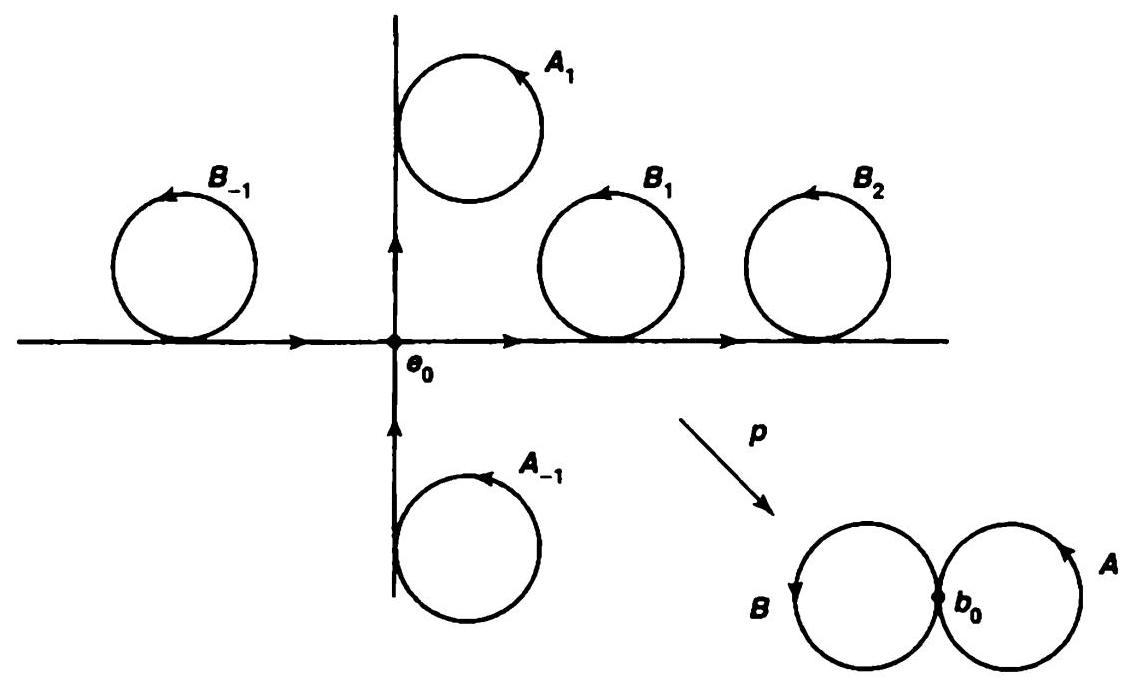
\includegraphics[width=1.0\textwidth]{images/81.2.jpg}
\end{center}
\hspace*{3em}

Figure 81.2
\end{example}
\end{centeredblock}

There is a method for constructing covering spaces that automatically leads to a covering that is regular; and in fact every \index{Regular covering space}regular covering space can be constructed by this method. It involves the action of a group \(G\) on a space \(X\) .

\begin{definition}
	Let \(X\) be a space, and let \(G\) be a subgroup of the group of homeomorphisms of \(X\) with itself. The \index{Orbit}orbit space \(X/G\) is defined to be the quotient space obtained from \(X\) by means of the equivalence relation \(x \sim  g\left( x\right)\) for all \(x \in  X\) and all \(g \in  G\) . The equivalence class of \(x\) is called the orbit of \(x\) .
\end{definition}

\begin{definition}
	If \(G\) is a group of homeomorphisms of \(X\) , the action of \(G\) on \(X\) is said to be \index{Properly discontinuous}properly discontinuous if for every \(x \in  X\) there is a neighborhood \(U\) of \(x\) such that \(g\left( U\right)\) is disjoint from \(U\) whenever \(g \neq  e\) . (Here \(e\) is the identity element of \(G\) .) It follows that \({g}_{0}\left( U\right)\) and \({g}_{1}\left( U\right)\) are disjoint whenever \({g}_{0} \neq  {g}_{1}\) , for otherwise \(U\) and \({g}_{0}^{-1}{g}_{1}\left( U\right)\) would not be disjoint.
\end{definition}

\begin{theorem}
	Let \(X\) be path connected and locally path connected; let \(G\) be a group of homeomorphisms of \(X\) . The quotient map \(\pi  : X \rightarrow  X/G\) is a covering map if and only if the action of \(G\) is properly discontinuous. In this case, the covering map \(\pi\) is regular and \(G\) is its group of covering transformations.
\end{theorem}

\begin{proof}
	We show \(\pi\) is an open map. If \(U\) is open in \(X\) , then \({\pi }^{-1}\pi \left( U\right)\) is the union of the open sets \(g\left( U\right)\) of \(X\) , for \(g \in  G\) . Hence \({\pi }^{-1}\pi \left( U\right)\) is open in \(X\) , so that \(\pi \left( U\right)\) is open in \(X/G\) by definition. Thus \(\pi\) is open.
Step 1. We suppose that the action of \(G\) is properly discontinuous and show that \(\pi\) is a covering map. Given \(x \in  X\) , let \(U\) be a neighborhood of \(x\) such that \({g}_{0}\left( U\right)\) and \({g}_{1}\left( U\right)\) are disjoint whenever \({g}_{0} \neq  {g}_{1}\) . Then \(\pi \left( U\right)\) is evenly covered by \(\pi\) . Indeed, \({\pi }^{-1}\pi \left( U\right)\) equals the union of the disjoint open sets \(g\left( U\right)\) , for \(g \in  G\) , each of which contains at most one point of each orbit. Therefore, the map \(g\left( U\right)  \rightarrow  \pi \left( U\right)\) obtained by restricting \(\pi\) is bijective; being continuous and open, it is a homeomorphism. The sets \(g\left( U\right)\) , for \(g \in  G\) , thus form a partition of \({\pi }^{-1}\pi \left( U\right)\) into slices.

Step 2. We suppose now that \(\pi\) is a covering map and show that the action of \(G\) is properly discontinuous. Given \(x \in  X\) , let \(V\) be a neighborhood of \(\pi \left( x\right)\) that is evenly covered by \(\pi\) . Partition \({\pi }^{-1}\left( V\right)\) into slices; let \({U}_{\alpha }\) be the slice containing \(x\) . Given \(g \in  G\) with \(g \neq  e\) , the set \(g\left( {U}_{\alpha }\right)\) must be disjoint from \({U}_{\alpha }\) , for otherwise, two points of \({U}_{\alpha }\) would belong to the same orbit and the restriction of \(\pi\) to \({U}_{\alpha }\) would not be injective. It follows that the action of \(G\) is properly discontinuous.

Step 3. We show that if \(\pi\) is a covering map, then \(G\) is its group of covering transformations and \(\pi\) is regular. Certainly any \(g \in  G\) is a covering transformation, for \(\pi  \circ  g = \pi\) because the orbit of \(g\left( x\right)\) equals the orbit of \(x\) . On the other hand, let \(h\) be a covering transformation with \(h\left( {x}_{1}\right)  = {x}_{2}\) , say. Because \(\pi  \circ  h = \pi\) , the points \({x}_{1}\) and \({x}_{2}\) map to the same point under \(\pi\) ; therefore there is an element \(g \in  G\) such that \(\mathrm{g}\left( {x}_{1}\right)  = {x}_{2}\) . The uniqueness part of Theorem 79.2 then implies that \(h = g\) .

It follows that \(\pi\) is regular. Indeed, for any two points \({x}_{1}\) and \({x}_{2}\) lying in the same orbit, there is an element \(g \in  G\) such that \(g\left( {x}_{1}\right)  = {x}_{2}\) . Then Corollary 81.3 applies.
\end{proof}
\begin{theorem}
	If \(p : X \rightarrow  B\) is a regular covering map and \(G\) is its group of covering transformations, then there is a homeomorphism \(k : X/G \rightarrow  B\) such that \(p = k \circ  \pi\) , where \(\pi  : X \rightarrow  X/G\) is the projection.
\end{theorem}

\begin{center}
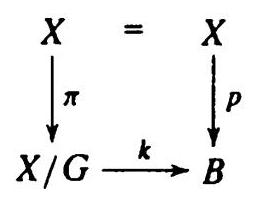
\includegraphics[width=0.2\textwidth]{images/81.25.jpg}
\end{center}
\hspace*{3em} 

\begin{proof}
	If \(g\) is a covering transformation, then \(p\left( {g\left( x\right) }\right)  = p\left( x\right)\) by definition. Hence \(p\) is constant on each orbit, so it induces a continuous map \(k\) of the quotient space \(X/G\) into \(B\) . On the other hand, \(p\) is a quotient map because it is continuous, surjective, and open. Because \(p\) is regular, any two points of \({p}^{-1}\left( b\right)\) belong to the same orbit under the action of \(G\) . Therefore, \(\pi\) induces a continuous map \(B \rightarrow  X/G\) that is an inverse for \(k\) .
\begin{centeredblock}
\begin{example}
	Let \(X\) be the cylinder \({S}^{1} \times  I\) ; let \(h : X \rightarrow  X\) be the homeomorphism \(h\left( {x,t}\right)  = \left( {-x,t}\right)\) ; and let \(k : X \rightarrow  X\) be the homeomorphism \(k\left( {x,t}\right)  = \left( {-x,1 - t}\right)\) . The groups \({G}_{1} = \{ e,h\}\) and \({G}_{2} = \{ e,k\}\) are isomorphic to the integers modulo 2; both act properly discontinuously on \(X\) . But \(X/{G}_{1}\) is homeomorphic to \(X\) , while \(X/{G}_{2}\) is homeomorphic to the Möbius band, as you can check. See Figure 81.3.

\begin{center}
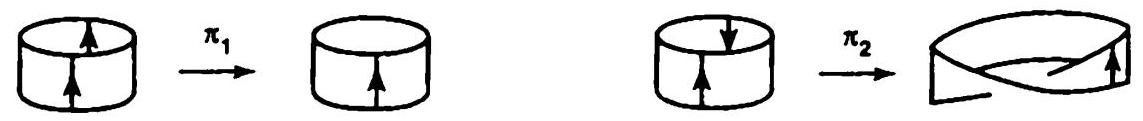
\includegraphics[width=1.0\textwidth]{images/81.3.jpg}
\end{center}
\hspace*{3em} 

Figure 81.3
\end{example}
\end{centeredblock}
\end{proof}
\section*{Exercises}
\begin{enumerate}[itemsep=0.4em, parsep=0pt, topsep=0pt, partopsep=0pt, leftmargin=*, label=\arabic*., ref=\arabic*]
\item
  \begin{enumerate}[itemsep=0.2em, parsep=0pt, topsep=0pt, partopsep=0pt, leftmargin=*, label=(\alph*), align=left]
  \item Find a group \(G\) of homeomorphisms of the torus \(T\) having order 2 such that \(T/G\) is homeomorphic to the torus.

  \item Find a group \(G\) of homeomorphisms of \(T\) having order 2 that \(T/G\) is homeomorphic to the Klein bottle.
  \end{enumerate}
\item Let \(X = A \vee  B\) be the wedge of two circles.
  \begin{enumerate}[itemsep=0.2em, parsep=0pt, topsep=0pt, partopsep=0pt, leftmargin=*, label=(\alph*), align=left]
  \item Let \(E\) be the space pictured in Figure 81.4; let \(p : E \rightarrow  X\) wrap each arc \({A}_{1}\) and \({A}_{2}\) around \(A\) and map \({B}_{1}\) and \({B}_{2}\) homeomorphically onto \(B\) . Show \(p\) is a regular covering map.
  \item Determine the group of covering transformations of the covering of \(X\) indicated in Figure 81.5 Is this covering regular? \begin{center} 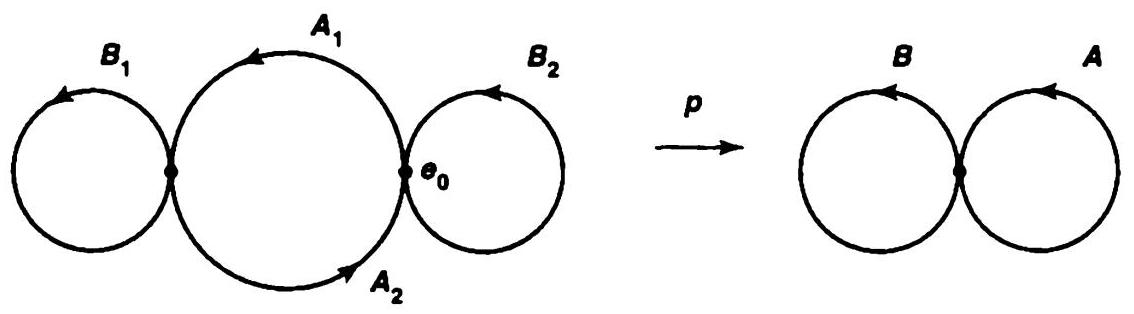
\includegraphics[width=1.0\textwidth]{images/81.4.jpg} \end{center} \hspace*{3em} Figure 81.4 \begin{center} 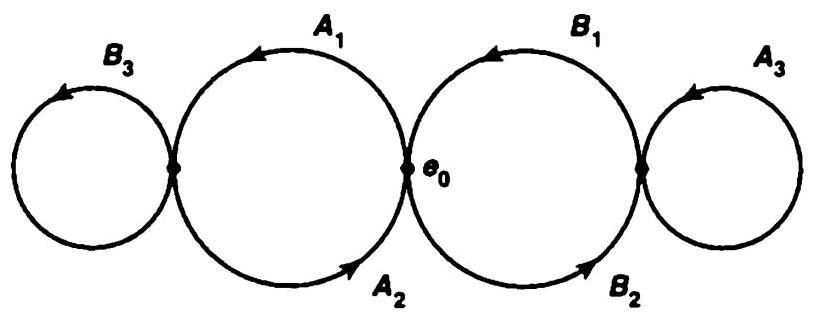
\includegraphics[width=0.7\textwidth]{images/81.5.jpg} \end{center} \hspace*{3em} Figure 81.5
  \item Repeat (b) for the covering pictured in Figure 81.6.
  \item Repeat (b) for the covering pictured in Figure 81.7. \begin{center} 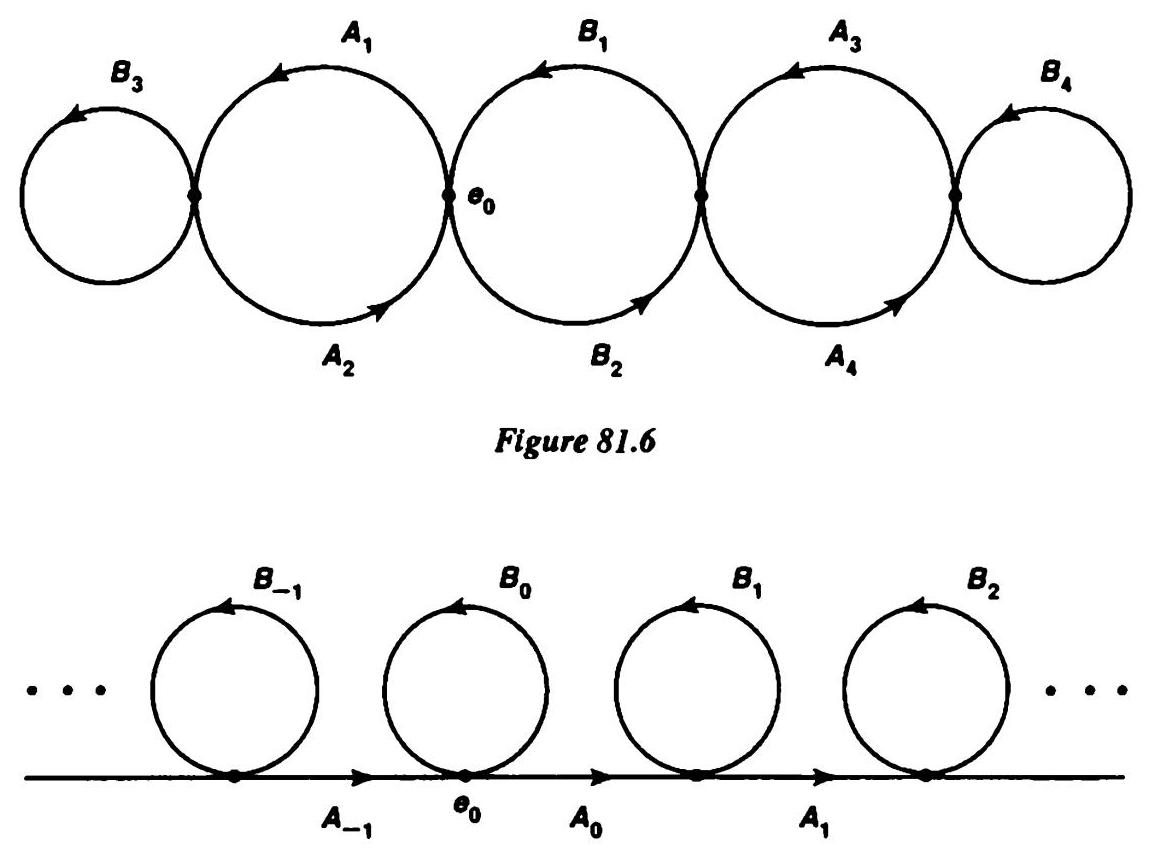
\includegraphics[width=1.0\textwidth]{images/81.6.jpg} \end{center} \hspace*{3em} Figure 81.7
  \end{enumerate}
\item Let \(p : X \rightarrow  B\) be a covering map (not necessarily regular); let \(G\) be its group of covering transformations.
  \begin{enumerate}[itemsep=0.2em, parsep=0pt, topsep=0pt, partopsep=0pt, leftmargin=*, label=(\alph*), align=left]
  \item Show that the action of \(G\) on \(X\) is properly discontinuous.
  \item Let \(\pi  : X \rightarrow  X/G\) be the projection map. Show there is a covering map \(k : X/G \rightarrow  B\) such that \(k \circ  \pi  = p\) . \begin{center} 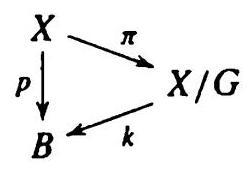
\includegraphics[width=0.2\textwidth]{images/81.7.jpg} \end{center} \hspace*{3em}
  \end{enumerate}
\item Let \(G\) be a group of homeomorphisms of \(X\) . The action of \(G\) on \(X\) is said to be fixed-point free if no element of \(G\) other than the identity \(e\) has a fixed point. Show that if \(X\) is Hausdorff, and if \(G\) is a finite group of homeomorphisms of \(X\) whose action is fixed-point free, then the action of \(G\) is properly discontinuous.
\item Consider \({S}^{3}\) as the space of all pairs of complex numbers \(\left( {{z}_{1},{z}_{2}}\right)\) satisfying the equation \({\left| {z}_{1}\right| }^{2} + {\left| {z}_{2}\right| }^{2} = 1\) . Given relatively prime positive integers \(n\) and \(k\) , define \(h : {S}^{3} \rightarrow  {S}^{3}\) by the equation \[ h\left( {{z}_{1},{z}_{2}}\right)  = \left( {{z}_{1}{e}^{{2\pi i}/n},{z}_{2}{e}^{{2\pi ik}/n}}\right) . \]
  \begin{enumerate}[itemsep=0.2em, parsep=0pt, topsep=0pt, partopsep=0pt, leftmargin=*, label=(\alph*), align=left]
  \item Show that \(h\) generates a subgroup \(G\) of the homeomorphism group of \({S}^{3}\) that is cyclic of order \(n\) , and that only the identity element of \(G\) has a fixed point. The orbit space \({S}^{3}/G\) is called the \index{Lens space}lens space \(L\left( {n,k}\right)\) .
  \item Show that if \(L\left( {n,k}\right)\) and \(L\left( {{n}^{\prime },{k}^{\prime }}\right)\) are homeomorphic, then \(n = {n}^{\prime }\) . [It is a theorem that \(L\left( {n,k}\right)\) and \(L\left( {{n}^{\prime },{k}^{\prime }}\right)\) are homeomorphic if and only if \(n = {n}^{\prime }\) and either \(k \equiv  {k}^{\prime }\left( {\;\operatorname{mod}\;n}\right)\) or \(k{k}^{\prime } \equiv  1\left( {\;\operatorname{mod}\;n}\right)\) . The proof is decidedly nontrivial.]
  \item Show that \(L\left( {n,k}\right)\) is a compact 3-manifold.
  \end{enumerate}
\item Prove the following: \textsl{Theorem.} Let \(X\) be a locally compact Hausdorff space; let \(G\) be a group of homeomorphisms of \(X\) such that the action of \(G\) is fixed-point free. Suppose that for each compact subspace \(C\) of \(X\) , there are only finitely many elements \(g\) of \(G\) such that the intersection \(C \cap  g\left( C\right)\) is nonempty. Then the action of \(G\) is properly discontinuous, and \(X/G\) is locally compact Hausdorff.  Proof.
  \begin{enumerate}[itemsep=0.2em, parsep=0pt, topsep=0pt, partopsep=0pt, leftmargin=*, label=(\alph*), align=left]
  \item For each compact subspace \(C\) of \(X\) , show that the union of the sets \(g\left( C\right)\) , for \(g \in  G\) , is closed in \(X\) . [Hint: If \(U\) is a neighborhood of \(x\) with \(\widetilde{U}\) compact, then \(\bar{U} \cup  C\) intersects \(g\left( {\bar{U} \cup  C}\right)\) for only finitely many \(g\) .]
  \item Show \(X/G\) is Hausdorff.
  \item Show the action of \(G\) is properly discontinuous.
  \item Show \(X/G\) is locally compact.
  \end{enumerate}
\end{enumerate}
\section*{§ 82 Existence of Covering Spaces}

We have shown that corresponding to each covering map \(p : E \rightarrow  B\) is a conjugacy class of subgroups of \({\pi }_{1}\left( {B,{b}_{0}}\right)\) , and that two such covering maps are equivalent if and only if they correspond to the same such class. Thus, we have an injective correspondence from equivalence classes of coverings of \(B\) to conjugacy classes of subgroups of \({\pi }_{1}\left( {B,{b}_{0}}\right)\) . Now we ask the question whether this correspondence is surjective, that is, whether for every conjugacy class of subgroups of \({\pi }_{1}\left( {B,{b}_{0}}\right)\) , there exists a covering of \(B\) that corresponds to this class.

The answer to this question is ``no,'' in general. In  \S 80, we gave an example of a path-connected, Iocally path-connected space \(B\) that had no simply connected covering space, that is, that had no covering space corresponding to the class of the trivial subgroup. This example relied on Lemma 80.4, which gave a condition that any space having a simply connected covering space must satisfy. We now introduce this condition formally.

\begin{definition}
	A space \(B\) is said to be \index{Semilocally simply connected}semilocally simply connected if for each \(b \in  B\) , there is a neighborhood \(U\) of \(b\) such that the homomorphism

\[
{i}_{ * } : {\pi }_{1}\left( {U,b}\right)  \rightarrow  {\pi }_{1}\left( {B,b}\right)
\]

induced by inclusion is trivial.
\end{definition}

Note that if \(U\) satisfies this condition, then so does any smaller neighborhood of \(b\) , so that \(b\) has ``arbitrarily small'' neighborhoods satisfying this condition. Note also that this condition is weaker than true \index{Local simple connectedness}local simple connectedness, which would require that within each neighborhood of \(b\) there should exist a neighborhood \(U\) of \(b\) that is itself simply connected.

Semilocal simple connectedness of \(B\) is both necessary and sufficient for there to exist, for every conjugacy class of subgroups of \({\pi }_{1}\left( {B,{b}_{0}}\right)\) , a corresponding covering space of \(B\) . Necessity was proved in Lemma 80.4; sufficiency is proved in this section.

\begin{theorem}
	Let \(B\) be path connected, locally path connected, and semilocally simply connected. Let \({b}_{0} \in  B\) . Given a subgroup \(H\) of \({\pi }_{1}\left( {B,{b}_{0}}\right)\) , there exists a covering map \(p : E \rightarrow  B\) and a point \({e}_{0} \in  {p}^{-1}\left( {b}_{0}\right)\) such that

\[
{p}_{ * }\left( {{\pi }_{1}\left( {E,{e}_{0}}\right) }\right)  = H
\]
\end{theorem}

\begin{proof}
	Step 1. Construction of \(E\) . The procedure for constructing \(E\) is reminiscent of the procedure used in complex analysis for constructing Riemann \index{surface with boundary@Surface with boundary}Surface with boundary surfaces. Let \(\mathcal{P}\) denote the set of all paths in \(B\) beginning at \({b}_{0}\) . Define an equivalence relation on \(\mathcal{P}\) by setting \(\alpha  \sim  \beta\) if \(\alpha\) and \(\beta\) end at the same point of \(B\) and
\[
\left\lbrack  {\alpha  * \bar{\beta }}\right\rbrack \in  H\text{ . }
\]

This relation is easily seen to be an equivalence relation. We will denote the equivalence class of the path \(\alpha\) by \({\alpha }^{\# }\) .

Let \(E\) denote the collection of equivalence classes, and define \(p : E \rightarrow  B\) by the equation

\[
p\left( {\alpha }^{\# }\right)  = \alpha \left( 1\right)
\]

Since \(B\) is path connected, \(p\) is surjective. We shall topologize \(E\) so that \(p\) is a covering map.

We first note two facts:

(1) If \(\left\lbrack  \alpha \right\rbrack = \left\lbrack  \beta \right\rbrack\) , then \({\alpha }^{\# } = {\beta }^{\# }\) .

(2) If \({\alpha }^{\# } = {\beta }^{\# }\) , then \({\left( \alpha  * \delta \right) }^{\# } = {\left( \beta  * \delta \right) }^{\# }\) for any path \(\delta\) in \(B\) beginning at \(\alpha \left( 1\right)\) .

The first follows by noting that if \(\left\lbrack  \alpha \right\rbrack = \left\lbrack  \beta \right\rbrack\) , then \(\left\lbrack  {\alpha  * \bar{\beta }}\right\rbrack\) is the identity element, which belongs to \(H\) . The second follows by noting that \(\alpha  * \delta\) and \(\beta  * \delta\) end at the same point of \(B\) , and

\[
\left\lbrack  {\left( {\alpha  * \delta }\right)  * \overline{\left( \beta  * \delta \right) }}\right\rbrack = \left\lbrack  {\left( {\alpha  * \delta }\right)  * \left( {\bar{\delta } * \bar{\beta }}\right) }\right\rbrack = \left\lbrack  {\alpha  * \bar{\beta }}\right\rbrack  ,
\]

which belongs to \(H\) by hypothesis.

Step 2. Topologizing \(E\) . One way to topologize \(E\) is to give \(\mathcal{P}\) the compact-open topology (see Chapter 7) and \(E\) the corresponding quotient topology. But we can topologize \(E\) directly as follows

Let \(\alpha\) be any element of \(\mathcal{P}\) , and let \(U\) be any path-connected neighborhood of \(\alpha \left( 1\right)\) . Define

\[
B\left( {U,\alpha }\right)  = \left\{  {{\left( \alpha  * \delta \right) }^{\# } \mid  \delta \text{ is a path in }U\text{ beginning at }\alpha \left( 1\right) }\right\}  .
\]

Note that \({\alpha }^{\# }\) is an element of \(B\left( {U,\alpha }\right)\) , since if \(b = \alpha \left( 1\right)\) , then \({\alpha }^{\# } = {\left( \alpha  * {e}_{b}\right) }^{\# }\) , this element belongs to \(B\left( {U,\alpha }\right)\) by definition. We assert that the sets \(B\left( {U,\alpha }\right)\) form a basis for a topology on \(E\) .

First, we show that if \({\beta }^{\# } \in  B\left( {U,\alpha }\right)\) , then \({\alpha }^{\# } \in  B\left( {U,\beta }\right)\) and \(B\left( {U,\alpha }\right)  = B\left( {U,\beta }\right)\) .

If \({\beta }^{\# } \in  B\left( {U,\alpha }\right)\) , then \({\beta }^{\# } = {\left( \alpha  * \delta \right) }^{\# }\) for some path \(\delta\) in \(U\) . Then

\[
\begin{aligned} {\left( \beta  * \bar{\delta }\right) }^{\# } = {\left( \left( \alpha  * \delta \right)  * \bar{\delta }\right) }^{\# }\;\text{ by (2) } &  \\ = {\alpha }^{\# }\;\text{ by }\left( 1\right) , &  \end{aligned}
\]

so that \({\alpha }^{\# } \in  B\left( {U,\beta }\right)\) by definition. See Figure 82.1. We show first that \(B\left( {U,\beta }\right)  \subset\)  \(B\left( {U,\alpha }\right)\) . Note that the general element of \(B\left( {U,\beta }\right)\) is of the form \({\left( \beta  * \gamma \right) }^{\# }\) , where \(\gamma\) is a path in \(U\) . Then note that

\[
\begin{aligned} {\left( \beta  * \gamma \right) }^{\# } = {\left( \left( \alpha  * \delta \right)  * \gamma \right) }^{\# } &  \\ = {\left( \alpha  * \left( \delta  * \gamma \right) \right) }^{\# }, &  \end{aligned}
\]

which belongs to \(B\left( {U,\alpha }\right)\) by definition. Symmetry gives the inclusion \(B\left( {U,\alpha }\right)  \subset\)  \(B\left( {U,\beta }\right)\) as well.

\begin{center}
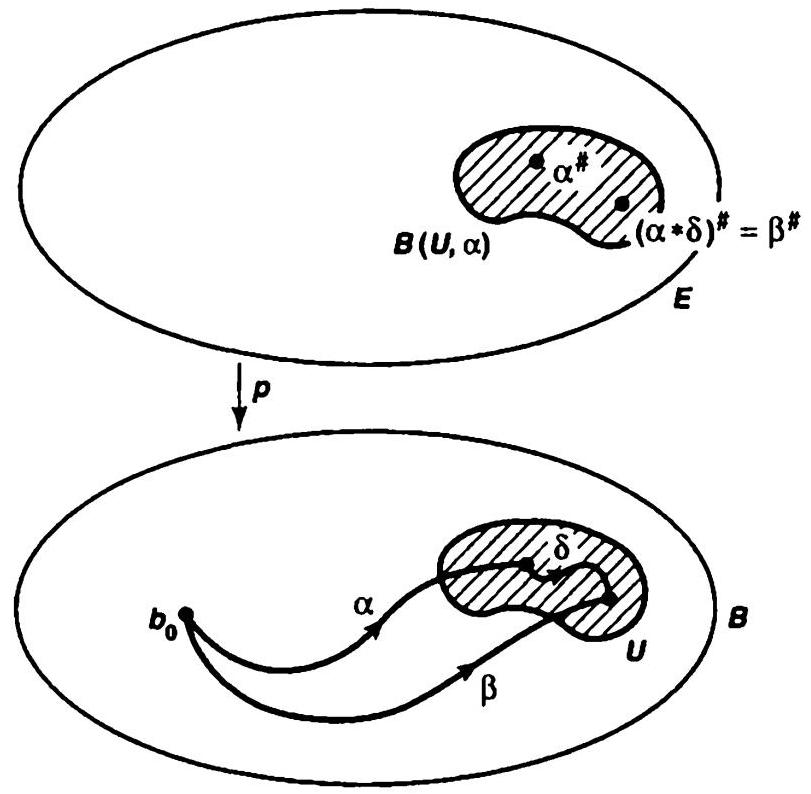
\includegraphics[width=0.7\textwidth]{images/82.1.jpg}
\end{center}
\hspace*{3em} 

Figure 82.1

Now we show the sets \(B\left( {U,\alpha }\right)\) form a basis. If \({\beta }^{\# }\) belongs to the intersection \(B\left( {{U}_{1},{\alpha }_{1}}\right)  \cap  B\left( {{U}_{2},{\alpha }_{2}}\right)\) , we need merely choose a path-connected neighborhood \(V\) of \(\beta \left( 1\right)\) contained in \({U}_{1} \cap  {U}_{2}\) . The inclusion

\[
B\left( {V,\beta }\right)  \subset  B\left( {{U}_{1},\beta }\right)  \cap  B\left( {{U}_{2},\beta }\right)
\]

follows from the definition of these sets, and the right side of the equation equals \(B\left( {{U}_{1},{\alpha }_{1}}\right)  \cap  B\left( {{U}_{2},{a}_{2}}\right)\) by the result just proved.

Step 3. The map \(p\) is continuous and open. It is easy to see that \(p\) is open, for the image of the basis element \(B\left( {U,\alpha }\right)\) is the open subset \(U\) of \(B\) : Given \(x \in  U\) , we choose a path \(\delta\) in \(U\) from \(\alpha \left( 1\right)\) to \(x\) ; then \({\left( \alpha  * \delta \right) }^{\# }\) is in \(B\left( {U,\alpha }\right)\) and \(p\left( {\left( \alpha  * \delta \right) }^{\# }\right)  = x\) .

To show that \(p\) is continuous, let us take an element \({\alpha }^{\# }\) of \(E\) and a neighborhood \(W\) of \(p\left( {\alpha }^{\# }\right)\) . Choose a path-connected neighborhood \(U\) of the point \(p\left( {\alpha }^{\# }\right)  = \alpha \left( 1\right)\) lying in \(W\) . Then \(B\left( {U,\alpha }\right)\) is a neighborhood of \({\alpha }^{\# }\) that \(p\) maps into \(W\) . Thus \(p\) is continuous at \({\alpha }^{\# }\) .

Step 4. Every point of \(B\) has a neighborhood that is evenly covered by \(p\) . Given \({b}_{1} \in  B\) , choose \(U\) to be a path-connected neighborhood of \({b}_{1}\) that satisfies the further condition that the homomorphism \({\pi }_{1}\left( {U,{b}_{1}}\right)  \rightarrow  {\pi }_{1}\left( {B,{b}_{1}}\right)\) induced by inclusion is trivial. We assert that \(U\) is evenly covered by \(p\) .

First, we show that \({p}^{-1}\left( U\right)\) equals the union of the sets \(B\left( {U,\alpha }\right)\) , as \(\alpha\) ranges over all paths in \(B\) from \({b}_{0}\) to \({b}_{1}\) . Since \(p\) maps each set \(B\left( {U,\alpha }\right)\) onto \(U\) , it is clear that \({p}^{-1}\left( U\right)\) contains this union. On the other hand, if \({\beta }^{\# }\) belongs to \({p}^{-1}\left( U\right)\) , then \(\beta \left( 1\right)  \in  U\) . Choose a path \(\delta\) in \(U\) from \({b}_{1}\) to \(\beta \left( 1\right)\) and let \(\alpha\) be the path \(\beta  * \bar{\delta }\) from \({b}_{0}\) to \({b}_{1}\) . Then \(\left\lbrack  \beta \right\rbrack = \left\lbrack  {\alpha  * \delta }\right\rbrack\) , so that \({\beta }^{\# } = {\left( \alpha  * \delta \right) }^{\# }\) , which belongs to \(B\left( {U,\alpha }\right)\) . Thus \({p}^{-1}\left( U\right)\) is contained in the union of the sets \(B\left( {U,\alpha }\right)\) .

Second, note that distinct sets \(B\left( {U,\alpha }\right)\) are disjoint. For if \({\beta }^{\# }\) belongs to \(B\left( {U,{\alpha }_{1}}\right)  \cap\)  \(B\left( {U,{\alpha }_{2}}\right)\) , then \(B\left( {U,{\alpha }_{1}}\right)  = B\left( {U,\beta }\right)  = B\left( {U,{\alpha }_{2}}\right)\) , by Step 2 .

Third, we show that \(p\) defines a bijective map of \(B\left( {U,\alpha }\right)\) with \(U\) . It follows that \(p \mid  B\left( {U,\alpha }\right)\) is a homeomorphism, being bijective and continuous and open. We already know that \(p\) maps \(B\left( {U,\alpha }\right)\) onto \(U\) . To prove injectivity, suppose that

\[
p\left( {\left( \alpha  * {\delta }_{1}\right) }^{\# }\right)  = p\left( {\left( \alpha  * {\delta }_{2}\right) }^{\# }\right) ,
\]

where \({\delta }_{1}\) and \({\delta }_{2}\) are paths in \(U\) . Then \({\delta }_{1}\left( 1\right)  = {\delta }_{2}\left( 1\right)\) . Because the homomorphism \({\pi }_{1}\left( {U,{b}_{1}}\right)  \rightarrow  {\pi }_{1}\left( {B,{b}_{1}}\right)\) induced by inclusion is trivial, \({\delta }_{1} * {\widetilde{\delta }}_{2}\) is path homotopic in \(B\) to the constant loop. Then \(\left\lbrack  {\alpha  * {\delta }_{1}}\right\rbrack = \left\lbrack  {\alpha  * {\delta }_{2}}\right\rbrack\) , so that \({\left( \alpha  * {\delta }_{1}\right) }^{\# } = {\left( \alpha  * {\delta }_{2}\right) }^{\# }\) , as desired.

It follows that \(p : E \rightarrow  B\) is a covering map in the sense used in earlier chapters. To show it is a covering map in the sense used in this chapter, we must show \(E\) is path connected. This we shall do shortly.

Step 5. Lufting a path in \(B\) . Let \({e}_{0}\) denote the equivalence class of the constant path at \({b}_{0}\) ; then \(p\left( {e}_{0}\right)  = {b}_{0}\) by definition. Given a path \(\alpha\) in \(B\) beginning at \({b}_{0}\) , we calculate its lift to a path \({mE}\) beginning at \({e}_{0}\) and show that this lift ends at \({\alpha }^{\# }\) .

To begin, given \(c \in  \left\lbrack  {0,1}\right\rbrack\) , let \({\alpha }_{c} : 1 \rightarrow  B\) denote the path defined by the equation

\[
{\alpha }_{c}\left( t\right)  = \alpha \left( {tc}\right) \;\text{ for }\;0 \leq  t \leq  1.
\]

Then \({\alpha }_{c}\) is the ``portion'' of \(\alpha\) that runs from \(\alpha \left( 0\right)\) to \(\alpha \left( c\right)\) . In particular, \({\alpha }_{0}\) is the constant path at \({b}_{0}\) , and \({\alpha }_{1}\) is the path \(\alpha\) itself. We define \(\widetilde{\alpha } : 1 \rightarrow  E\) by the equation

\[
\bar{\alpha }\left( c\right)  = {\left( {\alpha }_{c}\right) }^{\# }
\]

and show that \(\bar{\alpha }\) is continuous. Then \(\bar{\alpha }\) is a lift of \(\alpha\) , since \(p\left( {\bar{\alpha }\left( c\right) }\right)  = {\alpha }_{c}\left( 1\right)  = \alpha \left( c\right)\) ; furthermore, \(\widetilde{\alpha }\) begins at \({\left( {\alpha }_{0}\right) }^{\# } = {e}_{0}\) and ends at \({\left( {\alpha }_{1}\right) }^{\# } = {\alpha }^{\# }\) .

To verify continuity, we introduce the following notation. Given \(0 \leq  c < d \leq  1\) , let \({\delta }_{c,d}\) denote the path that equals the positive linear map of \(I\) onto \(\left\lbrack  {c,d}\right\rbrack\) followed by \(\alpha\) . Note that the paths \({\alpha }_{d}\) and \({\alpha }_{c} * {\delta }_{c,d}\) are path homotopic because one is just a reparametrization of the other. See Figure 82.2.

\begin{center}
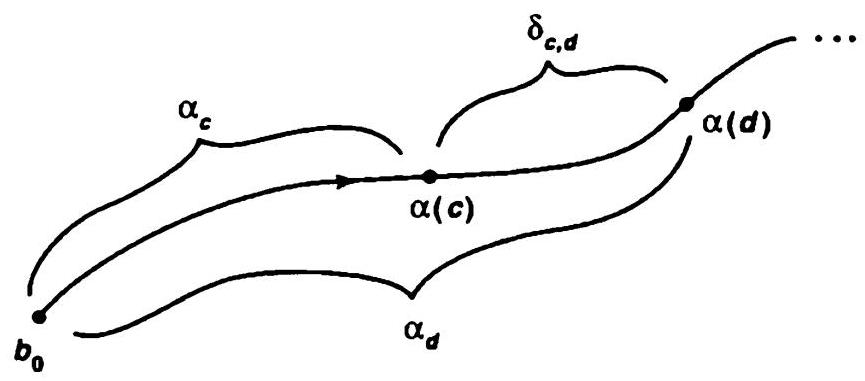
\includegraphics[width=0.8\textwidth]{images/82.2.jpg}
\end{center}
\hspace*{3em} 

Figure 82.2

We now verify continuity of \(\widetilde{\alpha }\) at the point \(c\) of \(\left\lbrack  {0,1}\right\rbrack\) . Let \(W\) be a basis element in \(E\) about the point \(\widetilde{\alpha }\left( c\right)\) . Then \(W\) equals \(B\left( {U,{\alpha }_{c}}\right)\) for some path-connected neighborhood \(U\) of \(\alpha \left( c\right)\) . Choose \(\epsilon  > 0\) so that for \(\left| {c - t}\right|  < \epsilon\) , the point \(\alpha \left( t\right)\) lies in \(U\) . We show that if \(d\) is a point of \(\left\lbrack  {0,1}\right\rbrack\) with \(\left| {c - d}\right|  < \epsilon\) , then \(\bar{\alpha }\left( d\right)  \in  W\) ; this proves continuity of \(\widetilde{\alpha }\) at \(c\) .

So suppose \(\left| {c - d}\right|  < \epsilon\) . Take first the case where \(d > c\) . Set \(\delta  = {\delta }_{c,d}\) ; then since \(\left\lbrack  {\alpha }_{d}\right\rbrack = \left\lbrack  {{\alpha }_{c} * \delta }\right\rbrack\) , we have

\[
\bar{\alpha }\left( d\right)  = {\left( {\alpha }_{d}\right) }^{\# } = {\left( {\alpha }_{c} * \delta \right) }^{\# }.
\]

Since \(\delta\) lies in \(U\) , we have \(\widetilde{\alpha }\left( d\right)  \in  B\left( {U,{\alpha }_{c}}\right)\) , as desired. If \(d < c\) , set \(\delta  = {\delta }_{d,c}\) and proceed similarly.

Step 6. The map \(p : E \rightarrow  B\) is a covering map. We need only verify that \(E\) is path connected, and this is easy. For if \({\alpha }^{\# }\) is any point of \(E\) , then the lift \(\bar{\alpha }\) of the path \(\alpha\) is a path in \(E\) from \({e}_{0}\) to \({\alpha }^{\# }\) .

Step 7. Finally, \(H = {p}_{ * }\left( {{\pi }_{1}\left( {E,{e}_{0}}\right) }\right.\) . Let \(\alpha\) be a loop in \(B\) at \({b}_{0}\) . Let \(\bar{\alpha }\) be its lift to \(E\) beginning at \({e}_{0}\) . Theorem 54.6 tells us that \(\left\lbrack  \alpha \right\rbrack \in  {p}_{ * }\left( {{\pi }_{1}\left( {E,{e}_{0}}\right) }\right)\) if and only if \(\bar{\alpha }\) is a loop in \(E\) . Now the final point of \(\widetilde{\alpha }\) is the point \({\alpha }^{\# }\) , and \({\alpha }^{\# } = {e}_{0}\) if and only if \(\alpha\) is equivalent to the constant path at \({b}_{0}\) , i.e., if and only if \(\left\lbrack  {\alpha  * {\bar{e}}_{{b}_{0}}}\right\rbrack \in  H\) This occurs precisely when \(\left\lbrack  \alpha \right\rbrack \in  H\) .
\end{proof}
\begin{corollary}
	The space \(B\) has a universal covering space if and only if \(B\) is path connected, locally path connected, and semilocally simply connected.
\end{corollary}

\section*{Exercises}
\begin{enumerate}[itemsep=0.4em, parsep=0pt, topsep=0pt, partopsep=0pt, leftmargin=*, label=\arabic*., ref=\arabic*]
\item Show that a simply connected space is semulocally simply connected.
\item Let \(X\) be the infinite earring in \({\mathbb{R}}^{2}\) . (See Example 1 of \( \S {80}\) .) Let \(C\left( X\right)\) be the subspace of \({\mathbb{R}}^{3}\) that is the union of all line segments joining points of \(X \times  0\) to the point \(p = \left( {0,0,1}\right)\) . It is called the cone on \(X\) . Show that \(C\left( X\right)\) is simply connected, but is not locally simply connected at the origin.
\end{enumerate}
\section*{* Supplementary Exercises: Topological Properties and \({\pi }_{1}\)}

The results of the preceding section tell us that the appropriate hypotheses for classifying the covering spaces of \(B\) are that \(B\) is path connected, locally path connected, and semilocally simply connected. We now show that they are also the correct hypotheses for studying the relation between various topological properties of \(B\) and the fundamental group of \(B\) .

1. Let \(X\) be a space; let \(\mathcal{A}\) be an open covering of \(X\) . Under what conditions does there exist an open covering \(\mathcal{B}\) of \(X\) refining \(\mathcal{A}\) such that for each pair \(B,{B}^{\prime }\) of elements of \(\mathcal{B}\) that have nonempty intersection, the union \(B \cup  {B}^{\prime }\) lies in an element of \(\mathcal{A}\) ?

(a) Show that such a covering \(\mathcal{B}\) exists if \(X\) is metrzable. [Hint: Choose \(\epsilon \left( x\right)\) so \(B\left( {x,{3\epsilon }\left( x\right) }\right)\) lies in an element of \(\mathcal{A}\) . Let \(\mathcal{B}\) consist of the open sets \(B\left( {x,\epsilon \left( x\right) }\right)\) .]

(b) Show that such a covering exists if \(X\) is compact Hausdorff. [Hint: Let \({A}_{1},\ldots ,{A}_{n}\) be a finite subcollection of \(\mathcal{A}\) that covers \(X\) . Choose an open covering \({C}_{1},\ldots ,{C}_{n}\) of \(X\) such that \({\bar{C}}_{i} \subset  {A}_{i}\) for each \(i\) . For each nonempty subset \(J\) of \(\{ 1,\ldots ,n\}\) , consider the set

\[
{B}_{J} = \mathop{\bigcap }\limits_{{j \in  J}}{A}_{j} - \mathop{\bigcup }\limits_{{j \notin  J}}{\bar{C}}_{j}.
\]

2. Prove the following:

\textsl{Theorem.}
	Let \(X\) be a space that is path connected, locally path connected, and semilocally simply connected. If \(X\) is regular with a countable basis, then \({\pi }_{1}\left( {X,{x}_{0}}\right)\) is countable.


\textsl{Proof.}
	Let \(\mathcal{A}\) be a covering of \(X\) by path-connected open sets \(A\) such that for each \(A \in  \mathcal{A}\) and each \(a \in  A\) , the homomorphism \({\pi }_{1}\left( {A,a}\right)  \rightarrow  {\pi }_{1}\left( {X,a}\right)\) induced by inclusion is trivial. Let \(\mathcal{B}\) be a countable open covering of \(X\) by nonempty path-connected sets that satisfies the conditions of Exercise 1. Choose a point \(p\left( B\right)  \in  B\) for each \(B \in  \mathcal{B}\) . For each pair \(B,{B}^{\prime }\) of elements of \(\mathcal{B}\) for which \(B \cap  {B}^{\prime } \neq  \varnothing\) , choose a path \(g\left( {B,{B}^{\prime }}\right)\) in \(B \cup  {B}^{\prime }\) from \(p\left( B\right)\) to \(p\left( {B}^{\prime }\right)\) . We call the path \(g\left( {B,{B}^{\prime }}\right)\) a select path.
Let \({B}_{0}\) be a fixed element of \(\mathcal{B}\) ; let \({x}_{0} = p\left( {B}_{0}\right)\) . Show that if \(f\) is a loop in \(X\) based at \({x}_{0}\) , then \(f\) is path homotopic to a product of select paths, as follows:

(a) Show that there is a subdivision

\[
0 = {t}_{0} < \cdots  < {t}_{n} = 1
\]

of \(\left\lbrack  {0,1}\right\rbrack\) such that \(f\) maps \(\left\lbrack  {{t}_{n - 1},{t}_{n}}\right\rbrack\) into \({B}_{0}\) , and for each \(i = 1,\ldots ,n - 1\) , \(f\) maps \(\left\lbrack  {{t}_{i - 1},{t}_{i}}\right\rbrack\) into an element \({B}_{i}\) of \(\mathcal{B}\) . Set \({B}_{n} = {B}_{0}\) .

(b) Let \({f}_{i}\) be the positive linear map of \(\left\lbrack  {0,1}\right\rbrack\) onto \(\left\lbrack  {{t}_{i - 1},{t}_{i}}\right\rbrack\) followed by \(f\) . Let \({g}_{i} = g\left( {{B}_{i - 1},{B}_{i}}\right)\) . Choose a path \({\alpha }_{i}\) in \({B}_{i}\) from \(f\left( {t}_{i}\right)\) to \(p\left( {B}_{i}\right)\) ; if \(\mathrm{i} = 0\) or \(n\) , let \({\alpha }_{i}\) be the constant path at \({x}_{0}\) . Show that

\[
\left\lbrack  {f}_{i}\right\rbrack * \left\lbrack  {\alpha }_{i}\right\rbrack = \left\lbrack  {\alpha }_{i - 1}\right\rbrack * \left\lbrack  {g}_{\iota }\right\rbrack  .
\]

(c) Show that \(\left\lbrack  f\right\rbrack = \left\lbrack  {g}_{1}\right\rbrack * \cdots  * \left\lbrack  {g}_{n}\right\rbrack\) .


3. Let \(p : E \rightarrow  X\) be a covering map such that \({\pi }_{1}\left( {X,{x}_{0}}\right)\) is countable. Show that if \(X\) is regular with a countable basis, so is \(E\) . [Hint: Let \(\mathcal{B}\) be a countable basis for \(X\) consisting of path-connected sets Let \(\mathcal{C}\) be the collection of path components of \({p}^{-1}\left( B\right)\) , for \(B \in  \mathcal{B}\) . Compare Exercise 6 of  \S 53.]

4. Prove the following:

\textsl{Theorem.}
	Let \(X\) be a space that is path connected, locally path connected, and semilocally simply connected. If \(X\) is compact Hausdorff, then \({\pi }_{1}\left( {X,{x}_{0}}\right)\) is finitely generated, and hence countable.


\textsl{Proof.}
	Repeat the proof outlined in Exercise 2, choosing \(\mathcal{B}\) to be finite. One has the equation
\[
\left\lbrack  f\right\rbrack = \left\lbrack  {g}_{1}\right\rbrack * \cdots  * \left\lbrack  {g}_{n}\right\rbrack  ,
\]

as before. Choose, for each \(x \in  X\) , a path \({\beta }_{x}\) from \({x}_{0}\) to \(x\) ; let \({\beta }_{{x}_{0}}\) be the constant path. If \(g = g\left( {B,{B}^{\prime }}\right)\) , define

\[
L\left( g\right)  = {\beta }_{x} * \left( {g * {\bar{\beta }}_{y}}\right) ,
\]

where \(x = p\left( B\right)\) and \(y = p\left( {B}^{\prime }\right)\) . Show that

\[
\left\lbrack  f\right\rbrack = \left\lbrack  {L\left( {g}_{1}\right) }\right\rbrack * \cdots  * \left\lbrack  {L\left( {g}_{n}\right) }\right\rbrack  .
\]

5. Let \(X\) be the infinite earnng (see Example 1 of  \S 80). Show that \(X\) is a compact Hausdorff space with a countable basis whose fundamental group is uncountable. [Hint: Let \({r}_{n} : X \rightarrow  {C}_{n}\) be a retraction. Given a sequence \({a}_{1},{a}_{2},\ldots\) of zeros and ones, show there exists a loop \(f\) in \(X\) such that, for each \(n\) , the element \({\left( {r}_{n}\right) }_{ * }\left\lbrack  f\right\rbrack\) is trivial if and only if \({a}_{n} = 0\) .]